\documentclass{article}
\usepackage[utf8]{inputenc}
\usepackage[italian]{babel}
\usepackage{graphicx}
\usepackage{multicol}
\usepackage{placeins}
\usepackage{tabularx}
\usepackage{multirow}
\usepackage{amsmath}
\usepackage{subcaption}
\usepackage{parskip}
\usepackage{csquotes}
\usepackage{textgreek}
\usepackage{changepage}
\usepackage{amssymb}
\usepackage{pifont}
\usepackage{titlesec}
\usepackage{eurosym}
\usepackage{amsmath,array,multicol}
\usepackage[a4paper, total={6in, 9in}]{geometry}
\newcommand{\beforesectiongap}{\vspace*{\baselineskip}}
\graphicspath{{./images/}}

% Scheda di testa di ogni attività sperimentale: rende immediatamente visibile
% l'orizzonte di simulazione usato, la domanda a cui l'attività risponde e l'esito.
\newcommand{\schedaattivita}[4]{%
\noindent
{\renewcommand{\arraystretch}{1.25}%
\begin{tabularx}{\linewidth}{|p{2.2cm}|X|}
\hline
\multicolumn{2}{|l|}{\textbf{Attività #1} \;,  \; orizzonte: \textbf{\textsc{#2}}} \\
\hline
\textbf{Domanda} & #3 \\
\hline
\textbf{Esito} & #4 \\
\hline
\end{tabularx}}\par\vspace{6pt}}

% Formattazione sezioni
\titleformat{\section}{\normalfont\Large\bfseries}{\thesection}{0.25em}{}
\setlength{\columnsep}{1cm}

% Colonna centrata
\newcolumntype{C}{>{\centering\arraybackslash}X}
\newcolumntype{Y}{>{\centering\arraybackslash}X}

% Titolo
\title{
\vspace*{-2cm}

\includegraphics[width=3cm]{logo.png} \\[0.5cm]
\textbf{Progetto PMCSN} \\[0.4cm]
\large \textbf{Gestione automatizzata delle richieste \\in farmacia tramite sistema Gollmann}
}
\author{
\textbf{Alessio Torroni}\\0365661
}
\date{\textit{Università degli studi di Roma Tor Vergata}}

\begin{document}

\maketitle
\begin{adjustwidth}{-0.5cm}{-0.5cm}
\section*{Abstract}

\begin{displayquote}
Il presente studio analizza un sistema reale di gestione delle richieste farmaceutiche
automatizzato, implementato in una farmacia dotata di robot Gollmann. Il sistema è modellato come
una rete di code con arrivi non stazionari, due Bracci robotici in concorrenza tra prelievi
cliente e rifornimenti, e un sottosistema di inventario a revisione periodica con politica
$(s,S)$ per cinque classi di farmaco. Obiettivo dello studio è la \textbf{riduzione dei costi di
esercizio a parità di qualità del servizio}, agendo su due leve operative,  la turnazione del
personale per fascia oraria e la politica di riordino delle scorte,  sotto il vincolo che le
perdite per \emph{out-of-stock} restino sotto il 5\%. Il confronto tra la gestione baseline e la
configurazione ottimizzata, condotto con simulazione a eventi discreti a orizzonte finito e
infinito, mostra un risparmio del 22\% circa sul costo giornaliero senza violare i vincoli di
servizio.
\end{displayquote}


\section*{Introduzione}
\begin{multicols}{2}
Negli ultimi anni le farmacie hanno iniziato a dotarsi di sistemi automatizzati di dispensazione
del farmaco per aumentare efficienza e precisione nel servizio. Il sistema analizzato in questo
studio prende come riferimento una farmacia dotata di robot Gollmann, con interfaccia diretta
verso le casse e capacità automatica di prelievo e carico.

Nel sistema reale, il personale gestisce due flussi principali di richieste:
\begin{itemize}
    \item[\ding{112}] clienti fisici, serviti da cinque casse collegate al robot,
    \item[\ding{112}] ordini online, gestiti da una cassa separata.
\end{itemize}
Le richieste, una volta inserite, vengono inoltrate a un dispatcher, che le smista ai due bracci
robotici Gollmann. Per evitare perdite legate alla mancata disponibilità di farmaci, è integrato
un sistema di inventario per classi di farmaco, con carico automatizzato attivato da alert e
gestito da due magazzinieri. I clienti fisici, ritirati i farmaci, saldano l'ordine presso le
casse di pagamento in uscita.

Il \emph{miglioramento atteso} non è
un'evoluzione dell'architettura, bensì la \textbf{riduzione dei costi operativi} del sistema
esistente, perseguita con la scelta ottima dei parametri gestionali e verificata
quantitativamente nel confronto finale.
\vspace{-1pt}
\subsection*{Termini Chiave}
Di seguito i termini chiave dello studio.

\begin{minipage}{\linewidth}
\centering
\begin{tabularx}{\linewidth}{|X|}
  \hline
  \textbf{Cliente fisico} \\
  \hline
  Utente che si presenta fisicamente in farmacia e viene servito da uno dei farmacisti al banco.\\
  \hline
\end{tabularx}
\end{minipage}

\begin{minipage}{\linewidth}
\centering
\begin{tabularx}{\linewidth}{|X|}
  \hline
  \textbf{Cliente Online} \\
  \hline
  Utente che effettua un ordine tramite e-commerce, gestito da un operatore dedicat.\\
  \hline
\end{tabularx}
\end{minipage}

\begin{minipage}{\linewidth}
\centering
\begin{tabularx}{\linewidth}{|X|}
  \hline
  \textbf{Dispatcher} \\
  \hline
  Sistema automatico che riceve gli ordini completati da tutte le casse e li instrada verso i due Bracci robotici Gollmann. \\
  \hline
\end{tabularx}
\end{minipage}

\begin{minipage}{\linewidth}
\centering
\begin{tabularx}{\linewidth}{|X|}
  \hline
  \textbf{Robot Gollmann} \\
  \hline
  Sistema robotico automatizzato che preleva i farmaci dagli scaffali interni al banco dei farmaci. \\
  \hline
\end{tabularx}
\end{minipage}

\begin{minipage}{\linewidth}
\centering
\begin{tabularx}{\linewidth}{|X|}
  \hline
  \textbf{Braccio Due} \\
  \hline
    Braccio robotico dotato di una singola coda, alimentata dal dispatcher, dedicato esclusivamente alle richieste dei clienti (nessun rifornimento).\\
  \hline
\end{tabularx}
\end{minipage}

\begin{minipage}{\linewidth}
\centering
\begin{tabularx}{\linewidth}{|X|}
  \hline
  \textbf{Braccio Uno} \\
  \hline
    Braccio robotico dotato di due code distinte: una per le richieste dei clienti provenienti dal dispatcher e una per il carico merci proveniente dal magazzino. \\
  \hline
\end{tabularx}
\end{minipage}

\begin{minipage}{\linewidth}
\centering
\begin{tabularx}{\linewidth}{|X|}
  \hline
  \textbf{Inventory system} \\
  \hline
   Sistema che tiene traccia del livello di scorte per classi di farmaci e genera alert periodici automatici in caso di superamento della soglia minima. \\
  \hline
\end{tabularx}
\end{minipage}

\begin{minipage}{\linewidth}
\centering
\begin{tabularx}{\linewidth}{|X|}
  \hline
  \textbf{Magazziniere} \\
  \hline
   Figura che interviene in risposta agli alert generati dall'inventory system ad ogni revisione periodica delle scorte, caricando i prodotti nel modulo di carico del robot. \\
  \hline
\end{tabularx}
\end{minipage}

\begin{minipage}{\linewidth}
\centering
\begin{tabularx}{\linewidth}{|X|}
  \hline
  \textbf{Cassa Pagamento} \\
  \hline
   Postazione in uscita (due sportelli) presso cui i clienti fisici saldano l'ordine dopo il prelievo robotizzato. I clienti online, che hanno già pagato, non vi transitano. \\
  \hline
\end{tabularx}
\end{minipage}
\end{multicols}
\vspace{-2pt}

\begin{figure}[h]
    \centering
    \includegraphics[width=1\linewidth]{images/alto_livello.png}
    \caption{Descrizione del sistema ad alto livello}
\end{figure}

\begin{multicols}{2}
\section{Scopi e Obiettivi}
\vspace{-1pt}
Trattandosi di un sistema \emph{già esistente e operativo}, lo studio non mira a modificarne
l'architettura, bensì a \textbf{valutarne le prestazioni} e a \textbf{ottimizzarne la gestione
operativa a costo minimo}. L'obiettivo primario è la \textbf{riduzione dei costi di esercizio a
parità di qualità del servizio}: si vuole individuare il modo più economico di far funzionare la
farmacia senza degradare l'esperienza del cliente e senza mettere a rischio la stabilità del
cuore automatizzato del sistema, i due bracci.

\subsubsection*{I costi in gioco e i rischi da governare}
Ogni \emph{out-of-stock} (OOS) è una \textbf{vendita persa}, dunque una perdita economica diretta. Contenere gli OOS richiede scorte
adeguate, ma tenerle richiede a sua volta rifornimenti frequenti, che caricano i Bracci robotici.

Ed è proprio il carico sui Bracci il punto delicato. Una domanda eccessiva ai bracci, generata
sia dai prelievi cliente sia dai rifornimenti, espone a \textbf{tre problemi distinti}:
\begin{itemize}
    \item[\ding{112}] \textbf{out-of-stock}: se il braccio non riesce a ricaricare le scorte al
    ritmo con cui vengono consumate, il banco si svuota e crescono le vendite perse;
    \item[\ding{112}] \textbf{perdita della stazionarietà}: se il tasso di arrivo al braccio supera
    il suo tasso di servizio ($\lambda > \mu$), la coda cresce illimitatamente e il sistema non
    raggiunge uno stato stazionario ma una condizione di collasso operativo;
    \item[\ding{112}] \textbf{aumento eccessivo dei tempi di risposta}: anche restando stabile
    ($\lambda < \mu$), avvicinandosi alla saturazione i tempi di attesa esplodono (andamento
    $\rho/(1-\rho)$), degradando la qualità del servizio e traducendosi anch'essi in una perdita
    (clienti insoddisfatti, minore capacità di smaltire la giornata).
\end{itemize}
Poiché i Bracci sono \textbf{una risorsa fisica non aumentabile}, non
si può risolvere il problema aggiungendo serventi: occorre \emph{governare il flusso} che li
raggiunge.

Lo studio agisce quindi su due leve che non alterano il sistema fisico:
\begin{itemize}
    \item[\ding{112}] la \textbf{politica di riordino $(s,S)$} delle scorte a banco, per classe di
    farmaco, che regola \emph{quanto} e \emph{quando} rifornire (e quindi il livello di OOS e il
    carico di rifornimento sui bracci);
    \item[\ding{112}] la \textbf{turnazione del personale} (farmacisti alle casse e magazzinieri)
    per fascia oraria, in funzione della domanda istantanea.
\end{itemize}
Il ruolo delle casse merita una precisazione. Le casse sono il punto d'ingresso
obbligato dei clienti e fungono da \textbf{regolatore (contingentamento) del flusso} verso i
bracci: con \emph{meno casse attive} i job raggiungono i Bracci a frequenza più bassa, riducendo il carico di picco a valle e allontanando i tre rischi
appena descritti; per contro, \emph{meno casse} significa più attesa in coda alle casse, quindi un
\textbf{tempo di risposta più alto}. Ridurre il personale, inoltre, abbatte il costo dominante di
esercizio. La turnazione delle casse è dunque una leva a doppio taglio, che agisce
contemporaneamente sul costo, sulla regolarità del flusso ai Bracci e sul tempo d'attesa del
cliente.

\subsubsection*{L'obiettivo}
L'obiettivo dello studio è trovare il \textbf{miglior compromesso} tra tutte queste tensioni:
minimizzare il costo totale giornaliero $C_{tot}$: 
\[
C_{tot} = C_{\text{personale}} + C_{\text{giacenza}} + C_{\text{shortage}} + C_{\text{ordini}},
\]
mantenendo gli out-of-stock sotto una soglia accettabile, garantendo la stazionarietà di tutti i
centri e non lasciando degenerare il tempo di risposta. Ogni leva sposta l'equilibrio: soglie di
riordino più alte riducono gli OOS ma aumentano giacenza e carico di rifornimento; meno casse
tagliano i costi e regolarizzano il flusso ai Bracci ma allungano l'attesa. Il punto ottimo è la
combinazione di $(s,S)$ e staffing che minimizza il costo complessivo rispettando i vincoli di
servizio.

\end{multicols}

\begin{table}[ht]
\centering
\begin{tabularx}{1\textwidth}{|X|>{\centering\arraybackslash}m{1.6cm}|}
  \hline
  Le perdite per mancanza di scorte (\emph{out of stock}) devono essere mantenute sotto la soglia & \vspace{1mm}5\%\vspace{1mm} \\
  \hline
  Il tempo di risposta end-to-end del cliente non deve peggiorare in modo significativo rispetto alla gestione baseline & \vspace{1mm}--\vspace{1mm} \\
  \hline
\end{tabularx}
\end{table}

\subsubsection*{QoS: Quality of Service}
\begin{table}[ht]
\centering
\begin{tabularx}{1\textwidth}{|X|}
  \hline
  Ridurre i costi di esercizio senza peggiorare in modo significativo le prestazioni percepite dal cliente (tempo di risposta), senza superare il vincolo sull'out-of-stock e senza compromettere la stabilità dei centri. \\
  \hline
\end{tabularx}
\end{table}
\newpage
\begin{multicols}{2}
\section{Modello concettuale}
Il sistema di gestione delle richieste farmaceutiche può essere modellato come una rete di code,
costituita da diversi centri operativi: casse, dispatcher, Bracci robotici Gollmann, casse di
pagamento e magazziniere, più un sistema di inventario che ne governa le scorte. I clienti sono
suddivisi in due categorie:
\begin{itemize}
    \item[\ding{112}]  Clienti fisici, che si presentano direttamente in farmacia;
    \item[\ding{112}]  Clienti online, che effettuano ordini tramite piattaforma e-commerce.
\end{itemize}

Per poter ricevere i farmaci, un cliente,  indipendentemente dal canale di provenienza,  deve
prima essere preso in carico da una cassa.

Nel dettaglio, i clienti fisici affluiscono in una coda unica, in cui vengono serviti da cinque
farmacisti secondo politica FIFO (first-in, first-out). I clienti online affluiscono invece in una
seconda coda separata, gestita da una sesta postazione dedicata.

Un ordine può contenere \textbf{più farmaci, anche di classi diverse}: il numero $K$ di farmaci
richiesti e la classe di ciascun farmaco sono attributi dell'ordine, estratti al suo ingresso nel
sistema. Al completamento del servizio al banco (fisico oppure online), l'ordine viene inviato al
dispatcher, che rappresenta il nodo di smistamento del sistema.

Una scelta strutturale di questo studio è che l'ordine attraversi la rete come \textbf{un unico
job}: la richiesta di $K$ farmaci non genera $K$ job distinti, ma entra nel \emph{tempo di
servizio} del braccio robotico, che deve eseguire $K$ prelievi consecutivi dall'inventario, modellando la richiesta come operazione atomica. 

Il dispatcher è modellato come una coda a servente singolo, con scheduling FIFO. Una volta
completato il breve servizio di smistamento, l'\emph{intero ordine} è instradato verso uno dei due
Bracci robotici:

- \textbf{Braccio Uno}, dotato di due code proprie, nelle quali confluiscono sia le richieste dei
clienti sia i rifornimenti provenienti dal magazzino;

- \textbf{Braccio Due}, dotato di una singola coda, nella quale confluiscono esclusivamente le
richieste dei clienti.

La logica di smistamento del dispatcher è uno \emph{scheduling probabilistico a probabilità
fisse}: un ordine cliente è inviato al Braccio Uno con probabilità $p_{b1}=0{,}20$ e al Braccio
Due con probabilità $p_{b2}=0{,}80$. Nei \textbf{primi 10 minuti di ogni ciclo di revisione delle
scorte} (ciclo da 30 minuti) il dispatcher instrada inoltre il 100\% dei clienti al Braccio Due
(\emph{finestra protetta}), lasciando il Braccio Uno dedicato ai soli rifornimenti appena
generati dalla revisione.

Il \textbf{Braccio Uno} si distingue per la doppia funzionalità: oltre a servire le richieste dei
clienti, gestisce il carico delle scorte provenienti dal magazzino. Per questo dispone di due code
distinte:
\begin{itemize}
    \item[\ding{112}] una per le richieste cliente, alimentata dal dispatcher;
    \item[\ding{112}] una per le richieste di carico, alimentata dal magazziniere.
\end{itemize}
La disciplina tra le due code è a \textbf{priorità non-preemptive}: un servizio in corso non viene
mai interrotto e, al completamento, si sceglie la coda da servire. La precedenza è assegnata ai
\textbf{prelievi cliente}: un carico di rifornimento (che movimenta molte confezioni ed è quindi
lungo) attende che non vi siano clienti in coda. La motivazione è duplice: (i) i pochi ordini
cliente instradati al Braccio Uno non devono accodarsi dietro carichi lunghi, così i loro tempi di
risposta restano allineati a quelli del Braccio Due; (ii) il rifornimento tollera l'attesa per
costruzione, perché le scorte a banco,  dimensionate dalla politica $(s,S)$,  fungono da
buffer di disaccoppiamento tra domanda e carico.

Al completamento del prelievo, i clienti \textbf{fisici} proseguono verso la \textbf{Cassa
Pagamento} (coda unica, due sportelli) per il saldo, e quindi escono dal sistema; i clienti
\textbf{online}, che hanno già pagato al momento dell'ordine, escono direttamente dal braccio.

\subsubsection*{Inventario, rifornimenti e out-of-stock}
Per monitorare la disponibilità dei prodotti nel robot è presente un inventory system per classi
di farmaco, ognuna gestita secondo un modello $(s, S)$ a revisione periodica. Le classi
considerate sono cinque: 
\begin{itemize}
\item \emph{Farmaci con ricetta}
\item \emph{Farmaci da banco (SOP/OTC)}
\item \emph{Integratori}
\item \emph{Dispositivi medici}
\item \emph{Preparazioni galeniche}
\end{itemize}

Ogni 60 minuti l'inventory system rivede i livelli: se la disponibilità di una classe è scesa
sotto la soglia minima $s$, genera un ordine di rifornimento che riporta la scorta al livello
massimo $S$ (politica \emph{order-up-to}); per ciascuna classe può essere pendente \textbf{un solo
ordine} alla volta. L'ordine è preso in carico dal magazziniere che, prelevato e spacchettato il
collo dal magazzino interno, lo immette nella coda di carico del Braccio Uno. Il carico a banco è
\textbf{incrementale}: le $Q$ confezioni di un rifornimento diventano disponibili una alla volta
durante il servizio di carico, non in blocco alla sua conclusione,  come avviene fisicamente, 
così un prelievo concorrente può già attingere alle unità caricate.

Nonostante l'inventory system, si considerano eventi di perdita per \textbf{out-of-stock}: se al
momento del prelievo un farmaco dell'ordine non è disponibile a banco, quel singolo articolo è
perso (il cliente rinuncia all'articolo, l'ordine prosegue con gli altri). La politica è quindi
\emph{lost-sales}: la domanda insoddisfatta non è arretrata (nessun backorder),  in farmacia il
cliente non attende, acquista altrove. La metrica di servizio dell'inventario è la
probabilità di out-of-stock per articolo, $P(\text{OOS}) = \text{articoli persi}/\text{articoli
domandati}$.

\subsection*{Stato del Sistema}
Le seguenti variabili rappresentano ad alto livello lo stato del sistema:

\begin{minipage}{\linewidth}
\centering
\begin{tabularx}{\linewidth}{|X|}
  \hline
  \textbf{Stato di ciascuna coda} \\
  \hline
   empty (vuota)\\
  \hline
   not empty (non vuota)\\
  \hline
\end{tabularx}
\end{minipage}

\begin{minipage}{\linewidth}
\centering
\begin{tabularx}{\linewidth}{|X|}
  \hline
  \textbf{Stato di ciascun servente dei centri con una singola coda} \\
  \hline
   idle (libero)\\
  \hline
   busy (occupato)\\
  \hline
\end{tabularx}
\end{minipage}

\begin{minipage}{\linewidth}
\centering
\begin{tabularx}{\linewidth}{|X|}
  \hline
  \textbf{Stato del servente del centro con due code (Braccio Uno)} \\
  \hline
   idle (libero)\\
  \hline
   busy\_p (occupato da un prelievo cliente)\\
  \hline
   busy\_c (occupato da un carico di rifornimento)\\
  \hline
\end{tabularx}
\end{minipage}

\begin{minipage}{\linewidth}
\centering
\begin{tabularx}{\linewidth}{|X|}
  \hline
  \textbf{Inventario (per ciascuna delle 5 classi)} \\
  \hline
   livello di scorta corrente $l_c(t) \ge 0$\\
  \hline
   ordine pendente (assente / quantità residua)\\
  \hline
\end{tabularx}
\end{minipage}

\end{multicols}

Al livello delle specifiche, lo stato del sistema è riassunto dal vettore
\[
x(t) = \bigl(\, n_C,\; n_O,\; n_D,\; (n_{B1}^{p}, n_{B1}^{c}),\;
n_{B2},\; n_P,\; n_M,\; \mathbf{L}(t),\; \mathbf{O}(t),\; \varphi(t) \,\bigr)
\]
dove $n_X$ è il numero di job nel centro $X$ (in coda più in servizio):
\begin{itemize}
  \item $n_C$ Farmacisti (5 serventi eterogenei), $n_O$ Cassa Online, $n_D$ Dispatcher,
        $n_{B2}$ Braccio Due, $n_P$ Cassa Pagamento (2 serventi) e $n_M$ Magazziniere (2 serventi),
        con $n_X \in \mathbb{N}$;
  \item il Braccio Uno serve due classi a priorità non-preemptive, quindi ha due componenti:
        $n_{B1}^{p}$ (prelievi cliente) e $n_{B1}^{c}$ (richieste di carico);
  \item $\mathbf{L}(t)=(l_1,\dots,l_5)$, con $l_c \in \{0,\dots,S_c\}$ livello di scorta della classe
        $c$; la politica è \emph{lost-sales}, quindi $l_c \ge 0$;
  \item $\mathbf{O}(t)=(o_1,\dots,o_5)$, con $o_c$ quantità di riordino ancora pendente della classe
        $c$ ($o_c = 0$ se nessun ordine è in volo: un solo ordine pendente per classe);
  \item $\varphi(t)=\lfloor t/1800\rfloor \bmod 24 \in \{0,\dots,23\}$ è la fascia oraria corrente,
        rilevante nell'orizzonte finito per via degli arrivi non stazionari (NSPP).
\end{itemize}
Lo stato di ciascuna coda (\emph{empty}/\emph{not empty}) e di ciascun servente (\emph{idle}/\emph{busy})
si deriva dalla popolazione del centro: il numero di serventi occupati è $\min(n_X, m_X)$, con il
vincolo di consistenza per cui un servente è \emph{idle} solo se la sua coda è vuota. Una
precisazione è dovuta per le casse: poiché i cinque farmacisti hanno velocità diverse, per una
descrizione esatta occorre sapere \emph{quali} serventi sono occupati, non solo quanti; a livello
computazionale lo stato è infatti mantenuto per singolo servente, mentre per le leggi operazionali
(Little, utilizzazioni) è sufficiente la popolazione $n_X$. Lo stato cambia soltanto in
corrispondenza di un evento; gli eventi artificiali (campionamento, cambio fascia, revisione delle
scorte senza ordine) non alterano lo stato fisico del sistema.

Quanto descritto finora nel modello concettuale si può schematizzare nell'immagine che segue.
L'immagine mostra una specifica del precedente schema descrittivo ad alto livello.

\begin{adjustwidth}{-0.5cm}{-0.5cm}
\begin{figure}[h]
    \centering
    \includegraphics[width=1.\linewidth]{images/immagine.png}
\end{figure}

\end{adjustwidth}
\begin{multicols}{2}
\subsection*{Eventi}
Gli eventi considerati in tutti i centri del sistema sono:
\begin{itemize}
\item[\ding{112}]  Completamento del servizio di un job
\item[\ding{112}]  Cambio di fascia oraria
\end{itemize}
Altri eventi che possiamo considerare nel centro \textbf{``Farmacisti''} sono:
\begin{itemize}
    \item[\ding{112}] Arrivo di un nuovo job nella coda alle casse
\end{itemize}
Altri eventi che possiamo considerare nel centro \textbf{``Braccio Uno''} sono:
\begin{itemize}
\item[\ding{112}] Arrivo di un nuovo ordine cliente nella coda dei prelievi
\item[\ding{112}] Arrivo di un nuovo ordine di carico nella coda dei rifornimenti
\item[\ding{112}] Ingresso a banco di una singola confezione durante un carico (carico incrementale)
\item[\ding{112}] Perdita di un articolo per assenza del farmaco (out-of-stock)
\end{itemize}
Altri eventi che possiamo considerare nel centro \textbf{``Braccio Due''} sono:
\begin{itemize}
\item[\ding{112}] Arrivo di un nuovo ordine cliente nella coda dei prelievi
\item[\ding{112}] Perdita di un articolo per assenza del farmaco (out-of-stock)
\end{itemize}
Altri eventi che possiamo considerare nel sistema \textbf{``Banco dei Farmaci''} (Inventory
System) sono:
\begin{itemize}
\item[\ding{112}] Decremento della giacenza di una classe a seguito di un prelievo riuscito
\item[\ding{112}] Revisione periodica delle scorte con eventuale generazione dell'ordine di
riordino (al superamento della soglia minima $s$)
\item[\ding{112}] Ricezione di una consegna dal magazziniere con conseguente incremento della
giacenza (una confezione alla volta)
\end{itemize}
Inoltre, nei centri \textbf{``Dispatcher''}, \textbf{``Cassa Online''}, \textbf{``Cassa
Pagamento''} e \textbf{``Magazziniere''} possiamo considerare come evento l'arrivo di un nuovo
job.

\subsection*{Descrizione degli Eventi}
Di seguito si descrivono brevemente gli eventi che governano la dinamica della simulazione
(modellata come simulazione ad eventi discreti):
\begin{itemize}
\item[\ding{112}] \textbf{ARRIVAL}: arrivo di un job presso un centro. Per i centri d'ingresso
(Casse, Cassa Online) deriva dal processo di Poisson non omogeneo esterno; per i centri interni
deriva dall'instradamento del dispatcher, dei Bracci o del magazziniere.
\item[\ding{112}] \textbf{DEPARTURE}: completamento del servizio di un job presso un centro e suo
eventuale instradamento al centro successivo secondo la matrice di routing.
\item[\ding{112}] \textbf{TIMECHANGE}: cambio di fascia oraria (ogni 30 minuti) con conseguente
aggiornamento dell'intensità di arrivo $\lambda(t)$.
\item[\ding{112}] \textbf{SLOTCHANGE}: revisione periodica delle scorte da parte dell'inventory
system ed eventuale generazione degli ordini di rifornimento. È un \emph{evento artificiale}:
se nessuna classe è sotto soglia non altera lo stato fisico.
\item[\ding{112}] \textbf{RESTOCK}: ingresso a banco di una singola confezione durante il servizio
di carico del Braccio Uno (carico incrementale); aggiorna il livello di scorta della classe.
\item[\ding{112}] \textbf{COMPLETION}: chiusura dell'ordine cliente verso la cassa d'origine al
termine del percorso.
\item[\ding{112}] \textbf{SAMPLING}: evento tecnico di campionamento usato per il calcolo delle
statistiche di finestra (artificiale, non altera lo stato).
\end{itemize}
\end{multicols}

\section*{Analisi spese e profitti}
\begin{multicols}{2}
L'analisi economica del sistema mette in relazione i \emph{costi} di esercizio con le
\emph{perdite} dovute al mancato servizio, allo scopo di confrontare le configurazioni operative
su un'unica scala monetaria (\euro/giorno).

\subsubsection*{Componenti di costo}
\begin{itemize}
    \item \textbf{Costo del personale}: costo orario medio lordo aziendale di
    \textbf{26 \euro/h per farmacista} (cassa) e \textbf{18 \euro/h per magazziniere},
    moltiplicato per le ore-persona effettivamente schedulate nella giornata. È la voce dominante
    (con 5 casse e 2 magazzinieri sempre attivi: $12\cdot(5\cdot26+2\cdot18) = 1\,992$
    \euro/giorno) ed è la leva principale di risparmio.
    \item \textbf{Costo di giacenza (holding)}: proporzionale al livello medio di scorta a banco
    \[C_{\text{giac}} = \sum_c h_c \cdot \bar{l}_c\]con $h_c$ derivato dal valore unitario della
    classe (tasso di immobilizzo $\approx 25\%$/anno): $h = \{0{,}0151,\ 0{,}0041,\ 0{,}0068,\
    0{,}0103,\ 0{,}0137\}$ \euro/unità/giorno per le classi 1--5.
    \item \textbf{Costo di OOS (shortage / lost-sales)}: ogni articolo perso per out-of-stock
    è una vendita persa, valorizzata con il margine unitario della classe:
    $p = \{8{,}8,\ 2{,}4,\ 4{,}0,\ 6{,}0,\ 8{,}0\}$ \euro/unità.
    \item \textbf{Costo amministrativo d'ordine}: $c = 2{,}5$ \euro{} per ordine di rifornimento
    emesso.
\end{itemize}
Per evitare doppi conteggi, la manodopera del magazziniere è contata \emph{una sola volta}, nel
costo del personale (turni): il costo d'inventario comprende solo giacenza, shortage e ordini.

\subsubsection*{Asimmetria dei costi d'inventario}
Il rapporto tra costo di shortage e costo di giacenza è dell'ordine di $p_c/h_c \approx 500$:
tenere a scaffale un'unità per un giorno costa centinaia di volte meno che perderne la vendita.
Ne discende una lettura importante per l'ottimizzazione: \textbf{l'inventario non è una leva di
costo},  non conviene mai barattare out-of-stock per risparmiare giacenza, e le
soglie $s$ vanno dimensionate per coprire la domanda durante il tempo di rifornimento, non
minimizzate. Il risparmio economico va cercato invece sul personale.

\subsubsection*{Funzione obiettivo}
La configurazione ottima è definita come quella che \textbf{minimizza il costo totale
giornaliero sotto i vincoli di servizio}:
\begin{gather*}
\min\; C_{tot} \\
\text{t.c.}\;\; P(\text{OOS}) \le 5\%, \quad
\mathbb{E}[T_{\text{s}}]\ \text{non degradato},
\end{gather*}
dove il costo di shortage già presente in $C_{tot}$ penalizza economicamente l'out-of-stock e il
vincolo del 5\% ne fissa il tetto. Si è \emph{deliberatamente evitato} uno ``score'' pesato
prestazioni/costo con pesi arbitrari: ogni dimensione del trade-off è portata in euro. Le scelte finali sono operate su \textbf{fronti di Pareto} costo--servizio, così che il
compromesso resti visibile e discutibile invece che nascosto in un peso.
\end{multicols}

\newpage

\section{Modello delle specifiche}


\section*{Farmacisti ($M/M/m$ a serventi eterogenei)}
\begin{multicols}{2}
\begin{itemize}
    \item[\ding{112}] Arrivi Markoviani nella coda alle postazioni dei Farmacisti: $\lambda_C(t) = 0{,}95\,\lambda(t)$ 
    \item[\ding{112}] Coda unica FIFO, $m=5$ serventi a velocità diverse
    \item[\ding{112}] Tempi di servizio esponenziali con medie eterogenee:
        \begin{itemize}
    \item Cassa 1: $\mathbb{E}[S_1] \approx 121{,}5 \ \text{s}$
    \item Cassa 2: $\mathbb{E}[S_2] \approx 148{,}6 \ \text{s}$
    \item Cassa 3: $\mathbb{E}[S_3] \approx 135{,}0 \ \text{s}$
    \item Cassa 4: $\mathbb{E}[S_4] \approx 162{,}1 \ \text{s}$
    \item Cassa 5: $\mathbb{E}[S_5] \approx 108{,}0 \ \text{s}$
    \end{itemize}
\end{itemize}

\vfill\null
\columnbreak
\vspace*{\fill}
\begin{center}
    \includegraphics[width=\linewidth]{images/immagine_farmacisti.png}
\end{center}
\vspace*{\fill}

\end{multicols}
\vspace{-2.5em}
\begin{multicols}{2}
Le postazioni dei Farmacisti sono modellate come un centro multi-server a coda unica con cinque serventi a
velocità diversa (serventi eterogenei): il servizio comprende l'accoglienza, la ricezione della
ricetta o della richiesta, l'inserimento dell'ordine a sistema e le indicazioni al cliente, con
durate medie diverse da farmacista a farmacista (esperienza, mansioni accessorie). Ciascun
servente ha tempo di servizio esponenziale con media propria: il sistema non è quindi un $M/M/m$
omogeneo e la dizione $M/M/m$ va intesa nel senso di multi-server markoviano con tassi di servizio
distinti. La scelta della distribuzione esponenziale,  che ha moda in zero, poco realistica per
un servizio con durata minima fisiologica,  è discussa e difesa quantitativamente nella sezione
di validazione, dove un test di sensitività mostra che la forma della distribuzione alle casse non
altera le conclusioni dello studio.

La farmacia osservata è operativa nella fascia oraria compresa tra le 08:00 e le 20:00 (12 ore,
43\,200 s); il flusso di arrivi è stato suddiviso in 24 intervalli temporali di 30 minuti, come
rappresentato nel grafico seguente.

Osservando l'andamento dei dati emergono picchi significativi nelle fasce di tarda mattinata
(11:30--12:30) e di sera (17:30--19:30), intervallati da periodi di minore affluenza (prime ore
del mattino, primo pomeriggio). Questa variabilità temporale,  con variazioni anche superiori al
100\% tra fasce contigue,  rende inadeguato un modello stazionario: il processo di arrivo è
quindi modellato come \textbf{processo di Poisson non omogeneo} (NSPP), con intensità $\lambda(t)$
costante a tratti sulle 24 fasce. La media giornaliera del profilo è $\bar{\lambda} = 0{,}018664$
req/s, pari a circa 800 clienti al giorno.

\end{multicols}
\begin{figure}[h]
    \centering
    \includegraphics[width=0.75\linewidth]{images/immagine_arrivi_medi.png}
\end{figure}
\beforesectiongap
\newpage
\begin{multicols}{2}
\section*{Cassa Online ($M/M/1$)}

\begin{itemize}
    \item[\ding{112}] Arrivi Markoviani di ordini online: $\lambda_{\text{online}}(t)=0{,}05\,\lambda(t)$
    \item[\ding{112}] Non è presente coda fisica di clienti, ma un flusso di richieste generate dal sito
    \item[\ding{112}] Tempi di servizio esponenziali con media $\mathbb{E}[S] = 60 \ \text{s}$
\end{itemize}

\columnbreak
\vspace*{\fill}
\begin{center}
    \includegraphics[width=0.8\linewidth]{images/immagine_casse_online.png}
\end{center}
\vspace*{\fill}
\end{multicols}
\begin{multicols}{2}
La cassa online è modellata come un sistema $M/M/1$: un singolo servente che processa
sequenzialmente gli ordini effettuati tramite il sito web della farmacia. Non rappresenta un punto
di accesso fisico, ma un canale alternativo attraverso cui una parte degli utenti inoltra le
proprie richieste da remoto.

Dall'osservazione dei dati, circa il \textbf{5\% degli arrivi giornalieri} proviene dal canale
online: a fronte di una media di $\approx 806$ arrivi totali al giorno, la cassa online gestisce
circa 40 ordini/giorno. La frazione è modellata con lo stesso processo di Poisson non omogeneo:
\[
\lambda_{\text{online}}(t) = 0{,}05 \, \lambda(t),
\]
ottenuto per assottigliamento (thinning) probabilistico del flusso esterno, che preserva la
proprietà di Poisson.

Il tempo di servizio è modellato come esponenziale con media $\mathbb{E}[S] = 60$ s: riflette la
natura del processo di evasione degli ordini online (verifica, conferma, predisposizione), fatto
di attività semplici e variabili che si prestano a un modello di durata senza memoria. Essendo un
$M/M/1$ in senso stretto, questo centro sarà usato come banco di prova esatto nella fase di
verifica.
\end{multicols}
\beforesectiongap
\begin{multicols}{2}
\section*{Dispatcher ($M/M/1$)}

\begin{itemize}
    \item[\ding{112}] Arrivi determinati dall'uscita dalle postazioni dei Farmacisti e dalla cassa online
    \item[\ding{112}] Tempo di servizio esponenziale: $\mathbb{E}[S] = 3 \ \text{s}$
    \item[\ding{112}] Funzione: instradare l'\emph{intero ordine} verso uno dei due bracci
    \item[\ding{112}] Smistamento probabilistico fisso ($p_{b1}=0{,}20$, $p_{b2}=0{,}80$) con
    finestra protetta di carico (primi 10 min di ogni ciclo da 30)
\end{itemize}

\columnbreak
\vspace*{\fill}
\begin{center}
    \includegraphics[width=0.7\linewidth]{images/immagine_dispatcher.png}
\end{center}
\vspace*{\fill}
\end{multicols}
\begin{multicols}{2}
Il dispatcher rappresenta un'unità logica software del sistema: riceve in ingresso gli ordini già
completati dalle postazioni dei Farmacisti e dalla cassa online, senza distinzione tra i due canali, e li
instrada ai bracci. Il suo tempo di servizio, $\mathbb{E}[S]=3$ s esponenziale, rappresenta un
processo automatizzato e regolare di smistamento; l'utilizzazione risultante è molto bassa e il
centro non è mai critico.

Il centro simula lo spacchettamento del singolo ordine in K richieste ai Bracci, che vengono evase in modo atomico. L'ordine all'atto pratico non viene spacchettato: il dispatcher per semplicità applica il routing una sola volta per ordine
e inoltra al braccio il job con i suoi attributi (numero di farmaci $K$, classi degli articoli,
canale di provenienza). Il numero di farmaci per ordine è modellato come
\[
K = \max\bigl(1,\ \mathrm{round}(\mathrm{Exp}(2{,}71))\bigr),
\qquad \mathbb{E}[K] \approx 2{,}86,
\]
cioè una esponenziale di media 2{,}71 arrotondata e forzata ad almeno un farmaco. La classe di ciascuno dei $K$ articoli è estratta con
probabilità statica stabilita a priori, sulla base di valutazioni della reale domanda delle classi di farmaci considerata.

\subsubsection*{Logica di smistamento}
Il dispatcher instrada ogni ordine cliente ai due Bracci secondo uno \textbf{scheduling
probabilistico} con probabilità fisse:
\[
p_{b1} = 0{,}20 \, \qquad p_{b2} = 0{,}80 \ .
\]
La quota verso Braccio Uno è deliberatamente bassa perché quel braccio è già impegnato dai
rifornimenti: come mostrato nel flusso forzato, il solo lavoro di carico assorbe circa il 74\%
della sua capacità alla domanda media, per cui quote cliente elevate lo renderebbero instabile.

\paragraph{Finestra protetta (carico).} Nei primi 10 minuti di ogni ciclo di revisione
delle scorte il dispatcher instrada il 100\% degli ordini cliente al Braccio
Due ($p_{b1}=0$ in quella finestra), così il Braccio Uno può smaltire senza concorrenza i carichi
generati dalla revisione appena avvenuta. Si tratta di un routing \emph{tempo-variante
deterministico} (schedulato), che mantiene noto il tasso d'ingresso di ciascun braccio per
intervallo. Mediando sul ciclo, la quota effettiva di ordini cliente al Braccio Uno è
\[
p_{b1}^{\text{eff}} = p_{b1}\cdot\tfrac{2}{3} \approx 0{,}133, \qquad
p_{b2}^{\text{eff}} \approx 0{,}867,
\]
valori usati nelle equazioni di traffico e verificati a posteriori sulle utilizzazioni misurate.

Essendo $p_{b1},p_{b2}$ probabilità di progetto note, l'instradamento ai Bracci rientra nello
scheduling astratto: il tasso d'ingresso a ciascun braccio è $\lambda_{\text{centro}} =
X_{\text{precedente}}\cdot p$, requisito necessario per l'analisi del flusso forzato e per la
validazione per centro.
\end{multicols}
\beforesectiongap

\section*{Braccio Uno (priorità non-preemptive, due code)}
\begin{multicols}{2}

\begin{itemize}
    \item[\ding{112}] Arrivi interni da \textit{Dispatcher} (ordini cliente) e da
    \textit{Magazziniere} (ordini di rifornimento)
    \item[\ding{112}] Due code distinte; disciplina a priorità \textit{non-preemptive} con
    precedenza ai \textbf{prelievi cliente} (FCFS intra-classe)
    \item[\ding{112}] Servizio \textbf{prelievo}: somma di $K$ estrazioni da normale troncata
    $\mathrm{TruncNormal}(10,\,5;\,[5,\,20])$ s,  una per farmaco, posizioni diverse
    \item[\ding{112}] Servizio \textbf{carico}: $Q$ volte \emph{una} estrazione da
    $\mathrm{TruncNormal}(15,\,5;\,[5,\,20])$ s,  $Q$ confezioni della stessa classe, stessa
    posizione
\end{itemize}

\columnbreak
\vspace*{\fill}
\begin{center}
    \includegraphics[width=\linewidth]{images/immagine_braccio_uno.png}
\end{center}
\vspace*{\fill}
\end{multicols}
\begin{multicols}{2}
Il \textbf{Braccio Uno} serve due flussi:
\begin{itemize}
    \item \textbf{ordini cliente} (prelievo di $K$ farmaci) dal \textit{Dispatcher};
    \item \textbf{ordini di rifornimento} dal \textit{Magazziniere} (ricostituzione delle scorte a
    banco).
\end{itemize}

Le due tipologie entrano in code separate. La disciplina è a priorità \textbf{non-preemptive}: un
servizio in corso non viene interrotto; al completamento, se è presente un ordine cliente in coda,
viene servito \emph{prima} di qualunque carico in attesa. All'interno di ciascuna coda vige
\textsc{FCFS}. La precedenza ai prelievi,  motivata nel modello concettuale,  è la scelta che
allinea i tempi di risposta dei clienti instradati a Braccio Uno con quelli del Braccio Due,
sfruttando il fatto che il rifornimento, per costruzione della politica $(s,S)$, tollera l'attesa.\\
Il tempo di servizio è \emph{generale} e \emph{compound}: per un prelievo è la somma di $K$
estrazioni indipendenti da normale troncata (i $K$ farmaci sono in $K$ posizioni diverse del
magazzino robotizzato), mentre per un carico le $Q$ confezioni,  della stessa classe, quindi
alla stessa posizione,  richiedono un tempo $Q$ volte \emph{una singola} estrazione: stessa
media per confezione, ma variabilità minore. Con troncatura per reiezione su $[5,20]$ s le medie
effettive per confezione risultano $\mathbb{E}[X_{\text{prel}}] \approx 11{,}1$ s e
$\mathbb{E}[X_{\text{car}}] \approx 13{,}9$ s.

\subsubsection*{Perché la normale troncata}
\begin{itemize}
    \item il limite inferiore (5 s) rappresenta il prelievo più rapido (farmaco vicino), quello
    superiore (20 s) il più lento (farmaco lontano/scomodo);
    \item la troncatura elimina durate irrealistiche mantenendo la variabilità dovuta a distanza a
    scaffale, micro-movimentazioni e verifiche;
    \item la forma unimodale con moda lontana da zero è adatta a task meccanici brevi e
    ripetitivi, a differenza dell'esponenziale.
\end{itemize}

\subsubsection*{Interazione con lo stock}
\begin{itemize}
    \item \textbf{Prelievi}: per ciascuno dei $K$ articoli dell'ordine viene richiesta un'unità
    della rispettiva classe; se la giacenza è a zero l'articolo è perso (\textsc{out-of-stock}
    per-articolo), l'ordine prosegue con gli altri.
    \item \textbf{Carichi}: le $Q$ unità incrementano la giacenza della classe \emph{una alla
    volta} durante il servizio (eventi \textsc{RESTOCK} equispaziati sul tempo di carico), come
    avviene fisicamente sul nastro: un prelievo concorrente può così attingere alle unità già
    caricate, riducendo gli out-of-stock ``di tempismo''.
\end{itemize}
Il servizio di carico resta un blocco unico ai fini di code e utilizzazione (il braccio è occupato
per l'intera durata); il carico incrementale cambia solo l'istante in cui le unità diventano
disponibili.
\end{multicols}

\beforesectiongap
\newpage
\section*{Braccio Due (coda unica, $M/G/1$)}
\begin{multicols}{2}

\begin{itemize}
    \item[\ding{112}] Arrivi interni solo dal \textit{Dispatcher} (ordini cliente)
    \item[\ding{112}] Una sola coda con disciplina \textsc{FCFS}
    \item[\ding{112}] Nessun carico/rifornimento dal \textit{Magazziniere}
    \item[\ding{112}] Servizio: somma di $K$ estrazioni da
    $\mathrm{TruncNormal}(15,\,5;\,[10,\,20])$ s, $\mathbb{E}[X]=15$ s per farmaco
    \item[\ding{112}] $\mathbb{E}[S_{B2}] = \mathbb{E}[K]\cdot 15 \approx 43$ s per ordine
    \item[\ding{112}] Integrazione con \textit{Inventory System} e out-of-stock per-articolo
\end{itemize}

\columnbreak
\vspace*{\fill}
\begin{center}
    \includegraphics[width=0.9\linewidth]{images/immagine_braccio_due.png}
\end{center}
\vspace*{\fill}
\end{multicols}
\begin{multicols}{2}
\subsubsection*{Ruolo e logica di servizio}
Il \textbf{Braccio Due} è dedicato esclusivamente al prelievo dei farmaci richiesti dai clienti.
A differenza del Braccio Uno non esegue operazioni di rifornimento, quindi non riceve traffico dal
Magazziniere e non necessita di priorità: tutti gli ordini entrano in un'unica coda servita
\textsc{FCFS}.

Il tempo di prelievo per confezione è modellato con la normale troncata
$\mathrm{TruncNormal}(15,5;[10,20])$,  troncatura simmetrica, media effettiva esattamente 15 s
,  e il servizio di un ordine è la somma di $K$ estrazioni indipendenti. La dizione $M/G/1$
riflette il servente singolo con servizio generale (compound); gli arrivi, pur essendo un flusso
interno filtrato dal routing, restano ben approssimati da un processo di Poisson, come confermato
in verifica dal confronto con la formula di Pollaczek--Khinchine.

Poiché riceve la quota prevalente del traffico cliente ($\approx 87\%$ effettivo) con un
\emph{unico} servente, il Braccio Due è il centro critico del percorso clienti: è il primo a
saturare all'aumentare di $\lambda$ sul flusso dei prelievi, ed è il motivo del cap sugli slot di
punta del profilo di arrivo. Durante le finestre protette assorbe il 100\% dei clienti e la sua
coda può allungarsi temporaneamente: è il prezzo, contenuto, pagato per dare respiro al carico del
Braccio Uno.

\subsubsection*{Interazione con stock e out-of-stock}
Come per il Braccio Uno, al servizio dell'ordine vengono richieste al banco le unità delle classi
dei $K$ articoli; ogni articolo non disponibile è conteggiato come out-of-stock (per-articolo)
mentre l'ordine prosegue. Al termine del prelievo l'ordine esce verso la Cassa Pagamento (clienti
fisici) o direttamente dal sistema (clienti online).
\end{multicols}
\beforesectiongap
\section*{Cassa Pagamento ($M/M/2$)}
\begin{multicols}{2}
\begin{itemize}
    \item[\ding{112}] Arrivi interni: clienti \textbf{fisici} in uscita dai Bracci (gli online
    saltano il centro)
    \item[\ding{112}] Coda unica, \textbf{2 sportelli}, disciplina \textsc{FCFS}
    \item[\ding{112}] Tempo di servizio esponenziale con media $\mathbb{E}[S] = 60$ s
    \item[\ding{112}] Uscita dal sistema al completamento del pagamento
\end{itemize}

La Cassa Pagamento chiude il percorso dei clienti fisici: ritirati i farmaci dal robot, il cliente
salda l'ordine presso uno dei due sportelli dedicati. Il servizio (conto, pagamento, scontrino,
eventuale busta) è modellato come esponenziale di media 60 s. I clienti online, che hanno già
pagato al momento dell'ordine, escono dal sistema direttamente dal braccio: il centro riceve
quindi il 95\% del flusso complessivo. Con due sportelli l'utilizzazione per servente resta
moderata ($\approx 0{,}54$ alla domanda media) e il centro non è critico; il suo contributo al
tempo di risposta end-to-end dei clienti fisici è però non trascurabile ($\approx 85$ s di
permanenza) ed è per questo incluso nel modello.
\end{multicols}
\beforesectiongap
\section*{Magazziniere ($M/G/2$, servizio proporzionale alla quantità)}

\begin{multicols}{2}

\begin{itemize}
    \item[\ding{112}] Arrivi interni dall'\textit{Inventory System} (ordini di rifornimento,
    spezzati in colli da al più 20 unità)
    \item[\ding{112}] Coda unica con $n=2$ serventi in parallelo
    \item[\ding{112}] Tempo di servizio \textbf{proporzionale alla quantità}:
    $S(Q) = \sum_{i=1}^{Q} \mathrm{Exp}(18)$,  circa 18 s di handling per confezione
    \item[\ding{112}] Uscita: l'ordine di carico, con la sua quantità $Q$, è instradato alla coda
    rifornimenti del \textbf{Braccio Uno}
\end{itemize}

\columnbreak
\vspace*{\fill}
\begin{center}
    \includegraphics[width=0.75\linewidth]{images/immagine_magazzinieri.png}
\end{center}
\vspace*{\fill}
\end{multicols}
\begin{multicols}{2}
\subsubsection*{Ruolo e logica di servizio}
Il \textbf{Magazziniere} è un centro multi-server a coda unica: riceve gli ordini di rifornimento
generati dalla revisione periodica delle scorte. Un riordino di quantità complessiva elevata viene
\textbf{spezzato in colli da al più 20 unità}, l'ordine \emph{logico} della classe resta uno solo, i colli ne sono la suddivisione operativa.

\subsubsection*{Tempo di servizio: perché $\propto Q$}
Il lavoro del magazziniere è fisicamente \emph{per confezione}: prelevato il collo (master carton)
dal magazzino interno, deve aprire il confezionamento di trasporto, estrarre e aprire i fardelli
terziari in cellophane (6--12 scatoline ciascuno), prelevare ogni singola scatolina, verificarla e
posarla sul nastro di carico. Il servizio è quindi modellato come somma di $Q$ tempi esponenziali
indipendenti di media 18 s,  il \emph{tempo medio di handling per confezione}, comprensivo delle
aperture ammortizzate,  e il servente resta occupato per l'intera durata. Un modello con tempo
per-ordine costante sottostimerebbe l'occupazione del magazziniere proprio sui riordini grandi.

\end{multicols}
\beforesectiongap
\newpage
\section*{Inventory System (politica $(s,S)$ per 5 classi, lost-sales)}
\begin{multicols}{2}
\begin{itemize}
    \item[\ding{112}] 5 classi di farmaco, capacità a banco $S = \{80,\,70,\,60,\,55,\,35\}$
    unità ($\sum_c S_c = 300$ = slot fisici del banco robotizzato)
    \item[\ding{112}] Politica $(R,s,S)$: revisione periodica ogni $R = 30$ minuti; se
    $l_c \le s_c$ si ordina $S_c - l_c$ (order-up-to)
    \item[\ding{112}] \textbf{Un solo ordine pendente per classe}
    \item[\ding{112}] \textbf{Lost-sales}: domanda insoddisfatta persa, $l_c(t) \ge 0$; metrica di
    servizio $P(\text{OOS})$ per articolo
    \item[\ding{112}] Domanda per classe proporzionale alla capacità:
    $P(\text{classe } c) = S_c / \sum S = \{26{,}7\%,\ 23{,}3\%,\ 20{,}0\%,\ 18{,}3\%,\ 11{,}7\%\}$
    \item[\ding{112}] Le soglie $s_c$ sono le \textbf{variabili di ottimizzazione} (le $S_c$ sono
    fisse, vincolate dalla capacità fisica)
\end{itemize}

Il sottosistema segue lo schema del \emph{Simple Inventory System} di Leemis--Park, con tre
estensioni che lo ancorano al sistema reale: (i) la \textbf{domanda non è un processo esogeno
indipendente} ma è generata dal flusso clienti simulato (compound: $K$ articoli per ordine,
multi-classe); (ii) il \textbf{lead time di consegna è endogeno}: emerge dal percorso
magazziniere $\to$ Braccio Uno (code e priorità comprese) invece che da una distribuzione
assegnata; (iii) la politica è \textbf{lost-sales} anziché backorder, coerente con il contesto
farmacia. Per la scelta lost-sales il livello non scende mai sotto zero e la shortage
time-averaged è nulla per costruzione: la metrica di servizio è la probabilità di out-of-stock
per articolo, vincolata al 5\%.

La revisione periodica è un evento artificiale schedulato (avviene anche quando non genera
ordini). Il periodo $R=30$ minuti è una variabile di controllo della politica: un $R$ più corto
riduce gli out-of-stock ma aumenta i costi amministrativi d'ordine; il confronto quantitativo
$R=30$ vs $R=60$ minuti è parte della ricerca di configurazione dell'inventario.

Come discusso nel modello di costo, l'asimmetria shortage/holding ($\approx 500\times$) rende
l'inventario un \emph{guardrail}: le soglie $s_c$ ottime sono le minime che coprono la domanda
della classe durante il lead time di rifornimento (più margine per le classi piccole, più
variabili in proporzione), non le massime possibili,  oltre la copertura del lead time
l'out-of-stock non scende più e si pagano solo giacenza e micro-riordini continui.
\end{multicols}

\section*{Matrice di Routing}

\noindent
\begin{minipage}[t]{0.48\textwidth}
\raggedright
Di seguito la matrice di routing del sistema:

\[
\mathbf{P}=
\bordermatrix{
           & \text{ext} & 1 & 2 & 3 & 4 & 5 & 6 & 7 \cr
\text{ext} & 0   & P_f & P_o & 0 & 0      & 0      & 0 & 0   \cr
1          & 0   & 0   & 0   & 1 & 0      & 0      & 0 & 0   \cr
2          & 0   & 0   & 0   & 1 & 0      & 0      & 0 & 0   \cr
3          & 0   & 0   & 0   & 0 & p_{b1} & p_{b2} & 0 & 0   \cr
4          & P_o & 0   & 0   & 0 & 0      & 0      & 0 & P_c \cr
5          & P_o & 0   & 0   & 0 & 0      & 0      & 0 & P_c \cr
6          & 0   & 0   & 0   & 0 & 1      & 0      & 0 & 0   \cr
7          & 1   & 0   & 0   & 0 & 0      & 0      & 0 & 0   \cr
}
\]

\begin{itemize}
    \item \textbf{ext}: Esterno
    \item \textbf{1}: Farmacisti
    \item \textbf{2}: Cassa Online
    \item \textbf{3}: Dispatcher
    \item \textbf{4}: Braccio Uno
    \item \textbf{5}: Braccio Due
    \item \textbf{6}: Magazziniere
    \item \textbf{7}: Cassa Pagamento
\end{itemize}

Il Magazziniere (nodo 6) riceve gli ordini di rifornimento $\lambda_{IS}$ generati
dall'Inventory System e instrada tutti i carichi verso il Braccio Uno (nodo 4, coda dedicata).
Dai Bracci (nodi 4 e 5) l'ordine prosegue verso la Cassa Pagamento se il cliente è fisico
(probabilità $P_c$), oppure esce dal sistema se il cliente è online (probabilità $P_o$); i
carichi di rifornimento serviti dal Braccio Uno terminano a banco (uscita dal punto di vista dei
job). La riga 4 della matrice si riferisce ai soli job cliente.

\subsubsection*{Parametri}
\begin{itemize}
    % 1. Aumenta lo spazio tra la fine di un punto e il successivo
    \setlength{\itemsep}{15pt} 
    
    % 2. Riduce lo spazio verticale generato in automatico da \[ ... \]
    \setlength{\abovedisplayskip}{3pt}
    \setlength{\belowdisplayskip}{3pt}
    \setlength{\abovedisplayshortskip}{3pt}
    \setlength{\belowdisplayshortskip}{3pt}

    \item $\mathbf{P_c}$: probabilità di entrare nel sistema accedendo alle postazioni dei Farmacisti
    \[ P_c = 0{,}95\]

   \item $\mathbf{P_o}$: probabilità di entrare nel sistema accedendo alla Cassa Online
    \[P_o = 1-P_c = 0{,}05\] 
    Un cliente, terminato il servizio alla cassa, raggiunge sempre il dispatcher (probabilità 1).

    \item $\mathbf{P_{b1}}$: probabilità di instradare un ordine cliente a Braccio Uno,
     \[P_{b1}=0{,}20\] 
     (quota effettiva $0{,}133$ per via della finestra protetta).

    \item $\mathbf{P_{b2}}$: probabilità di instradare un ordine cliente a Braccio Due, 
    \[P_{b2}=0{,}80\]
      (quota effettiva $0{,}867$).
\end{itemize}
\end{minipage}\hfill
\begin{minipage}[t]{0.48\textwidth}
\raggedright
Le intensità di arrivo cambiano per fascia oraria: si assume un flusso di richieste variabile e si
usa la matrice di routing per propagarne gli effetti sui centri interni.

\subsubsection{Arrivi per fascia oraria}
\begin{center}
\renewcommand{\arraystretch}{1.12}
\setlength{\tabcolsep}{6pt}
\begin{tabular}{|l|}
\hline
\textbf{$\lambda_i$ per ogni i-esima fascia oraria} \\ \hline
08:00 -- 08:30 $\Rightarrow\ \lambda_{1}=0{,}007050\,\text{req/s}$ \\ \hline
08:30 -- 09:00 $\Rightarrow\ \lambda_{2}=0{,}008615\,\text{req/s}$ \\ \hline
09:00 -- 09:30 $\Rightarrow\ \lambda_{3}=0{,}015500\,\text{req/s}$ \\ \hline
09:30 -- 10:00 $\Rightarrow\ \lambda_{4}=0{,}018335\,\text{req/s}$ \\ \hline
10:00 -- 10:30 $\Rightarrow\ \lambda_{5}=0{,}019800\,\text{req/s}$ \\ \hline
10:30 -- 11:00 $\Rightarrow\ \lambda_{6}=0{,}016200\,\text{req/s}$ \\ \hline
11:00 -- 11:30 $\Rightarrow\ \lambda_{7}=0{,}022200\,\text{req/s}$ \\ \hline
11:30 -- 12:00 $\Rightarrow\ \lambda_{8}=0{,}025500\,\text{req/s}^{\,(\ast)}$ \\ \hline
12:00 -- 12:30 $\Rightarrow\ \lambda_{9}=0{,}024935\,\text{req/s}$ \\ \hline
12:30 -- 13:00 $\Rightarrow\ \lambda_{10}=0{,}020400\,\text{req/s}$ \\ \hline
13:00 -- 13:30 $\Rightarrow\ \lambda_{11}=0{,}012900\,\text{req/s}$ \\ \hline
13:30 -- 14:00 $\Rightarrow\ \lambda_{12}=0{,}015765\,\text{req/s}$ \\ \hline
14:00 -- 14:30 $\Rightarrow\ \lambda_{13}=0{,}016135\,\text{req/s}$ \\ \hline
14:30 -- 15:00 $\Rightarrow\ \lambda_{14}=0{,}013200\,\text{req/s}$ \\ \hline
15:00 -- 15:30 $\Rightarrow\ \lambda_{15}=0{,}012000\,\text{req/s}$ \\ \hline
15:30 -- 16:00 $\Rightarrow\ \lambda_{16}=0{,}014665\,\text{req/s}$ \\ \hline
16:00 -- 16:30 $\Rightarrow\ \lambda_{17}=0{,}017700\,\text{req/s}$ \\ \hline
16:30 -- 17:00 $\Rightarrow\ \lambda_{18}=0{,}021635\,\text{req/s}$ \\ \hline
17:00 -- 17:30 $\Rightarrow\ \lambda_{19}=0{,}024000\,\text{req/s}$ \\ \hline
17:30 -- 18:00 $\Rightarrow\ \lambda_{20}=0{,}025500\,\text{req/s}^{\,(\ast)}$ \\ \hline
18:00 -- 18:30 $\Rightarrow\ \lambda_{21}=0{,}025500\,\text{req/s}^{\,(\ast)}$ \\ \hline
18:30 -- 19:00 $\Rightarrow\ \lambda_{22}=0{,}024900\,\text{req/s}$ \\ \hline
19:00 -- 19:30 $\Rightarrow\ \lambda_{23}=0{,}025500\,\text{req/s}$ \\ \hline
19:30 -- 20:00 $\Rightarrow\ \lambda_{24}=0{,}020000\,\text{req/s}$ \\ \hline
\multicolumn{1}{|l|}{\footnotesize $(\ast)$ slot di punta limitato al cap $0{,}0255$ req/s} \\ \hline
\end{tabular}
\end{center}
Media giornaliera del profilo: $\bar{\lambda} = 0{,}018664$ req/s ($\approx 806$ clienti/giorno);
media del profilo osservato prima del cap: $0{,}0190975$ req/s, usata come tasso costante di
riferimento nelle simulazioni a orizzonte infinito.
\end{minipage}

\newpage
\section{Modello computazionale}
\begin{multicols}{2}
Il modello è implementato in Java come \textbf{simulazione a eventi discreti} secondo il paradigma
\emph{next-event} (Leemis--Park): il tempo avanza da un evento al successivo estraendo dalla lista
degli eventi futuri quello con timestamp minimo, aggiornando lo stato e le statistiche integrate,
e programmando gli eventi conseguenti. Lo \emph{stato computazionale} comprende, oltre al vettore
di stato fisico $x(t)$ del modello concettuale, la lista degli eventi futuri e gli accumulatori
statistici: è l'informazione minima che consente di proseguire la run da un istante qualunque.

I tipi di evento coincidono con quelli descritti nel modello concettuale (\textsc{arrival},
\textsc{departure}, \textsc{timechange}, \textsc{slotchange}, \textsc{restock},
\textsc{completion}, \textsc{sampling}, più \textsc{abandon} presente ma mai schedulato). Ogni
centro è un oggetto che incapsula coda (o code), serventi e generazione del proprio tempo di
servizio; gli \emph{handler} degli eventi realizzano l'instradamento della matrice di routing e
l'interazione con l'inventory system. Le statistiche sono raccolte in due famiglie:
\emph{time-averaged} (aree integrate $\int X(t)\,dt$: popolazioni medie, utilizzazioni, livello
medio di scorta), aggiornate a ogni evento, e \emph{job-averaged} (tempi di risposta e di attesa),
accumulate al completamento dei job.

\subsubsection*{Generazione dei numeri casuali}
Si usa il generatore di \textbf{Lehmer} della libreria\texttt{Rngs}: $x_{i+1} = a\,
x_i \bmod m$ con $m = 2^{31}-1$ e moltiplicatore a periodo pieno $a = 48271$. Il generatore
fornisce \textbf{256 stream disgiunti} (jump multiplier $A_{256}=22925$), e la convenzione
adottata,  prescritta dal corso,  è \textbf{uno stream dedicato per ogni componente
stocastica}: arrivi esterni, scelta del canale fisico/online, classe di ciascun farmaco, numero
di farmaci $K$, instradamento ai bracci, e un tempo di servizio per ciascun centro (13 stream in
totale). Questo garantisce che le componenti siano statisticamente indipendenti e riproducibili, e
abilita l'uso dei \emph{common random numbers} nei confronti tra configurazioni.

\subsubsection*{Indipendenza delle repliche e dei batch}
Nell'orizzonte finito l'esperimento consiste in $n$ \textbf{repliche indipendenti} della giornata:
\texttt{plantSeeds} è chiamata \textbf{una sola volta, fuori dal loop} delle repliche, e ogni
replica prosegue dallo \emph{stato finale} degli stream della replica precedente. Le repliche
usano così sottosequenze disgiunte del generatore,  nessuna sovrapposizione, nessuna
correlazione indotta,  senza mai reinizializzare gli stream dentro il loop. Nell'orizzonte
infinito l'indipendenza (approssimata) è tra \emph{batch}: lo stato iniziale di un batch è lo
stato finale del precedente, e la decorrelazione è garantita dalla scelta della dimensione di
batch (sezione sulla calibrazione). Le stime intervallari usano in entrambi i casi la
t di Student con $\alpha = 0{,}05$.

Per ogni esperimento il programma scrive su file una serie per metrica e per centro (medie di
finestra con intervallo di confidenza nel finito, medie di batch nell'infinito), da cui sono
prodotti i grafici e le tabelle delle sezioni successive.
\end{multicols}



\newpage
\section{Verifica}
\begin{multicols}{2}
La verifica risponde alla domanda: \emph{il modello computazionale realizza correttamente il
modello delle specifiche?} Non potendo disporre di una forma chiusa dell'intera rete, la verifica
è condotta a pezzi, su quattro livelli: bilanci di conteggio, leggi operazionali, confronto
per-centro con i modelli analitici, e un test degenerato del sottosistema d'inventario.

\subsubsection*{Bilanci di conteggio}
In ogni esperimento valgono esattamente le identità di conservazione. Sui \emph{job}: arrivi  $=$ serviti. Sugli
\emph{articoli}: domandati $2\,324{,}11$ $=$ venduti $2\,232{,}62$ $+$ persi per out-of-stock
$91{,}49$; inoltre venduti $-$ caricati $=$ scorta iniziale $-$ scorta finale (il banco parte
pieno e chiude la giornata parzialmente scarico). Il rapporto articoli/clienti osservato,
$2\,324{,}11/810{,}22 = 2{,}868$, riproduce $\mathbb{E}[K] = 2{,}863$ del modello di input.

\subsubsection*{Leggi operazionali (Little)}
Il tempo di risposta di sistema è calcolato in \emph{tre modi indipendenti}: (A) somma dei tempi
per centro pesata sui flussi, (B) media dei tempi individuali ingresso--uscita, (C) legge di
Little applicata all'area integrata della popolazione ($\mathbb{E}[N]/X$). I tre stimatori
coincidono entro frazioni di punto percentuale in tutte le run,  una verifica incrociata che
copre contemporaneamente contatori, aree e timestamp.

\subsubsection*{Confronto con i modelli analitici per centro}
I centri markoviani della rete ammettono formule esatte, e per il Braccio Due,  servente singolo
con servizio generale,  vale Pollaczek--Khinchine:
\[
E[T_q] \;=\; \frac{\lambda\,\mathbb{E}[S^2]}{2\,(1-\rho)},
\]
dove i momenti del servizio compound $S=\sum_{i=1}^{K}X_i$ si ottengono analiticamente dai
parametri di input:
\[
\mathbb{E}[S] = \mathbb{E}[K]\,\mathbb{E}[X] = 42{,}95 \text{ s},
\]
\[
\mathbb{E}[S^2] = \mathbb{E}[K]\,\mathrm{Var}(X) + \mathbb{E}[K^2]\,\mathbb{E}[X]^2 \approx 3\,382
\text{ s}^2,
\]
con $\mathbb{E}[K]=2{,}863$, $\mathbb{E}[K^2]=14{,}94$, $\mathbb{E}[X]=15$ s,
$\mathrm{Var}(X)=7{,}28$ s$^2$ (normale troncata su $[10,20]$). Per la Cassa Pagamento
($M/M/2$) si usa la formula di Erlang-C; gli arrivi a valle dei Bracci non sono esattamente
poissoniani, quindi l'accordo atteso è approssimato. Il confronto usa la run a orizzonte infinito
di riferimento ($\lambda = 0{,}0190975$, 64 batch da 1024, intervalli al 95\%).
\end{multicols}

\begin{table}[ht]
\centering
\renewcommand{\arraystretch}{1.25}
\begin{tabular}{|l|l|l|c|c|}
\hline
\textbf{Centro} & \textbf{Modello} & \textbf{Metrica} & \textbf{Analitico} & \textbf{Simulato (IC 95\%)} \\
\hline
Cassa Online & $M/M/1$ & $\mathbb{E}[T]$ (s) & 63{,}65 & $63{,}80 \pm 2{,}01$ \\
             &         & $\mathbb{E}[N_q]$   & 0{,}0035 & $0{,}0031 \pm 0{,}0007$ \\
\hline
Dispatcher   & $M/M/1$ & $\mathbb{E}[T]$ (s) & 3{,}182 & $3{,}179 \pm 0{,}025$ \\
             &         & $\mathbb{E}[N_q]$   & 0{,}0035 & $0{,}0034 \pm 0{,}0002$ \\
\hline
Cassa Pagamento & $M/M/2$ (Erlang-C) & $\mathbb{E}[T]$ (s) & 85{,}3 & $84{,}20 \pm 2{,}00$ \\
                &                    & $\mathbb{E}[N_q]$   & 0{,}458 & $0{,}439 \pm 0{,}031$ \\
\hline
Braccio Due  & $M/G/1$ (P--K) & $\mathbb{E}[T]$ (s) & 139{,}7 & $138{,}51 \pm 6{,}39$ \\
\hline
\end{tabular}
\caption{Verifica per centro: valori analitici (dai parametri di input del modello) contro stime
di batch means. Tutti i valori analitici cadono negli intervalli di confidenza simulati.}
\end{table}

\begin{table}[ht]
\centering
\renewcommand{\arraystretch}{1.25}
\begin{tabular}{|l|c|c|}
\hline
\textbf{Centro} & $\rho$ \textbf{previsto (flusso forzato)} & $\rho$ \textbf{misurato (IC 95\%)} \\
\hline
Farmacisti & 0{,}490 & $0{,}4684 \pm 0{,}0050$ \\
Braccio Uno     & 0{,}816 & $0{,}8167 \pm 0{,}0073$ \\
Braccio Due     & 0{,}711 & $0{,}7053 \pm 0{,}0074$ \\
Magazziniere    & 0{,}492 & $0{,}4786 \pm 0{,}0040$ \\
Cassa Pagamento & 0{,}544 & $0{,}5433 \pm 0{,}0072$ \\
\hline
\end{tabular}
\caption{Utilizzazioni previste dal flusso forzato contro utilizzazioni misurate (orizzonte
infinito, $\lambda = 0{,}0190975$).}
\end{table}

\begin{multicols}{2}
L'accordo è entro l'intervallo di confidenza per Braccio Uno e Cassa Pagamento, ed entro il 3\%
per gli altri centri, con scarti spiegabili dal modello stesso. Per le \textbf{casse} la
previsione $0{,}490$ usa la media aritmetica dei cinque tempi di servizio (135 s), ma con serventi
\emph{eterogenei} i farmacisti più veloci completano più job dei lenti: il tempo di servizio
efficace pesato sull'uso è $\approx 129$ s e l'utilizzazione media ne risulta lievemente inferiore
,  è la sottigliezza per cui, con serventi a velocità diverse, la popolazione non basta e conta
\emph{quali} serventi sono occupati. Per il \textbf{magazziniere} lo scarto ($-2{,}7\%$)
corrisponde alla quota di domanda persa per out-of-stock ($\approx 2\%$), che non genera
rifornimento. La previsione del Braccio Uno,  costruita sommando lavoro di prelievo e di carico
,  centra il valore misurato: conferma sia le quote effettive di routing ($0{,}133/0{,}867$,
finestra protetta inclusa) sia il modello di lavoro ``una confezione caricata per unità
venduta''.

\subsubsection*{Test degenerato dell'inventario}
Il sottosistema d'inventario è la componente più articolata e meno standard del modello e proprio per questa ricchezza merita una verifica dedicata, capace di isolarne e certificarne la meccanica di base. L'idea è
ricondurre il nostro inventario, scegliendo opportunamente i parametri, a un modello di cui si
conosca già il comportamento esatto: il \emph{Simple Inventory System} descritto da Leemis e Park
(programma \texttt{Sis3}), riferimento canonico della letteratura per la politica $(s,S)$ a
revisione periodica.

Nel test l'inventario viene quindi fatto \emph{degenerare} a quel caso canonico. Lo si riduce a una
sola classe, gli si somministra una domanda di Poisson esogena e indipendente --- scollegata dalla
rete di code --- e lo si dota di una revisione periodica e di un lead time di consegna anch'esso
esogeno, campionato da una $U(0,1)$ come nel testo di riferimento. I parametri sono infine scelti in
modo che non si verifichi mai uno stockout, cosicché la nostra politica lost-sales e il backlogging
del modello di Leemis e Park producano necessariamente la stessa traiettoria: in queste condizioni i
due sistemi \emph{devono} coincidere non solo in media, ma realizzazione per realizzazione.

È in quest'ultimo dettaglio che il test diventa stringente. Anziché confrontare due medie
campionarie, si pilotano \textbf{entrambi} i modelli, il nostro \texttt{InventorySystem}
e un'implementazione fedele del loop di \texttt{Sis3}, con la \emph{stessa identica sequenza di
numeri casuali} (stesso generatore di Lehmer, stessi stream): a parità di realizzazione qualunque
differenza, per quanto piccola, sarebbe la firma di un errore nella meccanica e non un effetto del
caso. Il risultato è un accordo \textbf{esatto}: su tre diverse combinazioni di seed e parametri,
tutte le statistiche canoniche coincidono con scarto relativo nullo, e l'integrale di holding
risulta identico fino alla quarta cifra decimale.

Ciò che il test dimostra è dunque che la meccanica della politica $(s,S)$ è implementata
correttamente: la condizione di riordino, il ripristino \emph{order-up-to} fino alla soglia $S$, la
gestione dell'ordine pendente e l'integrazione temporale della giacenza. Restano fuori dal suo
raggio, per scelta, le dinamiche accoppiate che il caso degenere annulla di proposito.
\end{multicols}
\newpage
\section{Validazione}
\begin{multicols}{2}
La validazione risponde alla domanda complementare: \emph{il modello rappresenta adeguatamente il
sistema reale?} Conviene affrontarla distinguendo, tra i parametri del modello 
\textbf{misurati sul campo} da quelli assunti. Le tre sorgenti stocastiche dominanti ovvero, il
profilo degli arrivi dall'esterno, i tempi di servizio delle casse e i
tempi di servizio dei Bracci robotici provengono da \textbf{misurazioni condotte presso
una farmacia reale} dotata di sistema Gollmann; i restanti parametri sono invece \emph{assunzioni
ragionate}, coerenti con la logica operativa del sistema e con la letteratura.

Questa distinzione ha un peso metodologico. Gli input che governano il carico dei centri critici sono \emph{ancorati al
dato reale}, non inventati: il modello è dunque validato alla sorgente nelle sue componenti più
determinanti. Ciò che manca, e che non è stato possibile reperire, sono le \textbf{tracce di
servizio end-to-end} (i tempi reali di attraversamento, cliente per cliente) contro cui confrontare
direttamente l'\emph{output} della simulazione. In loro assenza la validazione dell'output si fonda
su quattro evidenze indirette: 
\begin{itemize}
    \item plausibilità dei valori a fronte dell'esperienza operativa
    \item coerenza del comportamento tra fasce orarie
    \item check di flusso del sottosistema d'inventario
    \item robustezza delle conclusioni rispetto alle assunzioni
\end{itemize}

\subsubsection*{Plausibilità e coerenza}
Alla domanda media il tempo end-to-end di un cliente fisico è di circa 6 minuti (di cui
$\approx 2{,}2$ alla cassa, $\approx 2{,}3$ al prelievo robotizzato, $\approx 1{,}4$ al
pagamento), le utilizzazioni dei centri restano sotto $0{,}85$ e le code si allungano nelle fasce
di punta per riassorbirsi in quelle successive; il comportamento qualitativo atteso da una
farmacia reale correttamente dimensionata. Il profilo degli arrivi, ricavato dall'osservazione
delle fasce orarie, riproduce i picchi di tarda mattinata e di sera con il calo della pausa
pranzo.
\end{multicols}
\subsubsection*{Coerenza al variare delle fasce orarie (controllo di consistenza)}
Un controllo di validazione classico, praticabile anche in assenza di tracce reali dell'output,
consiste nel verificare che il modello \emph{reagisca} al variare delle condizioni di carico nel
modo prescritto dalla teoria delle code: all'aumentare del tasso di arrivo, utilizzazioni, code e
tempi di risposta devono crescere. Il modello offre questo
test lungo la giornata stessa: è sufficiente tenere \emph{costante} la configurazione. Usiamo la
baseline, cinque casse in tutte le fasce, così che l'unica grandezza a cambiare da fascia a
fascia sia $\lambda(t)$, e osservare come si spostano le metriche. Confrontiamo la fascia più
scarica con quella di picco:

\begin{center}
\renewcommand{\arraystretch}{1.2}
\begin{tabular}{|l|c|c|c|c|c|}
\hline
\textbf{Fascia} & $\lambda$ (req/s) & interarrivo & $\rho_{\text{casse}}$ &
$\mathbb{E}[T]_{\text{sist}}$ & $\mathbb{E}[N_q]_{\text{casse}}$ \\
\hline
08:00--08:30 (scarica) & 0{,}0071 & $\approx 142$ s & 0{,}14 & 150 s & $\approx 0$ \\
11:30--12:00 (picco)   & 0{,}0255 & $\approx 39$ s  & 0{,}61 & 402 s & 0{,}44 \\
\hline
\end{tabular}
\end{center}

Passando dalla fascia calma a quella di picco il tasso di arrivo si moltiplica per $3{,}6$ e, come
atteso, \textbf{tutte le metriche peggiorano in modo coerente}: l'utilizzazione delle casse sale da
$0{,}14$ a $0{,}61$, la coda da $\approx 0$ a $0{,}44$ job in attesa, il tempo di risposta di
sistema da $150$ a $402$ s. La relazione è sistematica su tutte le 24 fasce: la correlazione tra
$\lambda(t)$ e l'utilizzazione delle casse è praticamente perfetta ($r = 0{,}997$, come impone
$U = X\,\mathbb{E}[S]$), mentre quella con il tempo di risposta è positiva ma più bassa
($r = 0{,}81$) perché il tempo di risposta eredita la \emph{memoria} della coda nelle fasce
serali risente dell'arretrato accumulato durante i picchi, che si riassorbe solo nelle fasce
successive a $\lambda$ più basso. 
\begin{multicols}{2}
\subsubsection*{Check di flusso dell'inventario}
A regime la politica order-up-to deve ricaricare tanto quanto vende: nelle run a orizzonte
infinito le unità ordinate eguagliano le unità domandate a meno della quota out-of-stock
($-1{,}7\%$), e nell'orizzonte finito la differenza tra venduto e caricato coincide con lo
svuotamento del banco tra inizio e fine giornata. Il \emph{delivery lag} misurato (dall'emissione
dell'ordine all'ultima confezione a banco) è in media $\approx 23$ minuti.La catena magazziniere--braccio smaltisce un ciclo di riordino entro il
ciclo successivo, coerentemente con il dimensionamento della politica.

\subsubsection*{Sensitività alla distribuzione di servizio delle casse}
La scelta esponenziale per il servizio delle postazioni dei farmacisti presta il fianco a una critica nota: l'onere
di un servizio reale ha una durata minima fisiologica, mentre l'esponenziale ha moda in zero. Per
quantificarne l'impatto è stato eseguito un test di sensitività a orizzonte infinito sostituendo
all'esponenziale una \textbf{Erlang-4 di pari media} (coefficiente di variazione da 1 a 0{,}5,
moda maggiore di zero):

\begin{center}
\renewcommand{\arraystretch}{1.2}
\begin{tabular}{|l|c|c|c|}
\hline
\textbf{Metrica} & \textbf{Exp} & \textbf{Erlang-4} & $\Delta$ \\
\hline
$\rho$ casse            & 0{,}468 & 0{,}468 & $\sim 0$ \\
$\mathbb{E}[N_q]$ casse & 0{,}095 & 0{,}071 & $-25\%$ \\
$W_q$ casse (s)         & 5{,}23  & 3{,}94  & $-25\%$ \\
$\mathbb{E}[T]$ sistema (s) & 357{,}8 & 354{,}8 & $-0{,}8\%$ \\
\hline
\end{tabular}
\end{center}

La lettura è triplice. Primo, l'utilizzazione è \emph{identica}: dipende solo dalla media del
servizio ($U = X\,\mathbb{E}[S]$, proprietà distribution-free), e il test lo conferma. Secondo, la coda delle casse si accorcia del 25\%, nella
direzione e nell'ordine di grandezza previsti dalla dipendenza di Pollaczek--Khinchine dal
coefficiente di variazione. Terzo, l'effetto
sul tempo di risposta \emph{di sistema} è nullo entro gli intervalli di confidenza ($-0{,}8\%$),
perché le casse lavorano a utilizzazione moderata e non sono il collo di bottiglia. I bracci,
che lo sono, adottano già normali troncate con moda lontana da zero, esenti dalla critica. Si
mantiene quindi l'esponenziale alle postazioni dei farmacisti: preserva la validazione markoviana in forma chiusa ed è
\emph{conservativa} (a parità di media sovrastima le attese se la variabilità reale è minore), con
la consapevolezza, che il bias cresce con l'utilizzazione e spinge
l'ottimizzazione dello staffing verso il sovra-servizio, mai verso il sotto-dimensionamento.
\end{multicols}

\newpage
\section{Il piano sperimentale}
\begin{multicols}{2}
La progettazione degli esperimenti è organizzata in \textbf{otto attività}, raggruppate in due fasi:
\begin{itemize}
    \item[\ding{112}] \textbf{Fase I,  il sistema attuale }: stabilire che il
    modello converge, tarare gli strumenti di misura dell'orizzonte infinito, e misurare costi e
    servizio della gestione baseline;
    \item[\ding{112}] \textbf{Fase II,  l'ottimizzazione }: scegliere la politica
    d'inventario e lo staff per fascia, ricomporre le scelte negli scenari ottimizzati e
    quantificare il confronto finale.
\end{itemize}
Ogni attività si apre con una \textbf{scheda} che ne dichiara l'\textbf{orizzonte di simulazione},
la domanda a cui risponde e l'esito: la distinzione tra i due orizzonti è il filo conduttore della trattazione.

\subsubsection*{Perché entrambi gli orizzonti, e con quali ruoli}
L'oggetto vero dello studio è la \textbf{giornata operativa}, e per questo l'orizzonte di
riferimento è quello \textbf{finito}: la farmacia apre alle 08:00 con il sistema vuoto e il banco
pieno, lavora dodici ore con un tasso di arrivo che cambia di fascia in fascia, e chiude. Le
condizioni iniziali e la non stazionarietà non sono un disturbo da eliminare, ma parte del fenomeno
che vogliamo misurare. È in questo contesto che hanno senso le domande operative
dello studio: quanti farmacisti tenere in ciascuna fascia, quale probabilità di out-of-stock si
osserva sulla giornata, quanto costa la giornata. Metodologicamente la giornata è una simulazione
terminante, che si analizza con \textbf{repliche indipendenti}: ripetiamo la giornata $n = 128$
volte, ogni replica fornisce un'osservazione $\bar{x}_i(\tau)$, e da queste ricaviamo la media
d'ensemble e l'intervallo di confidenza con la t di Student a $n-1$ gradi di libertà. Baseline,
scenari ottimizzati e confronto finale vivono tutti su questo orizzonte.

L'\textbf{orizzonte infinito} entra in gioco per un compito ben preciso e circoscritto:
\textbf{scegliere il numero di casse e magazzinieri da assegnare a ciascuna fascia oraria}. La
difficoltà è che nella giornata reale le fasce si susseguono e si influenzano a vicenda,
(l'arretrato di una si riversa sulla successiva) rendendo difficile isolare il merito di una
singola scelta di staffing. Per aggirare l'ostacolo si ``congela'' una fascia e la si fa durare per
sempre: si tiene il suo $\lambda$ costante e si porta il sistema a regime, dimenticate le condizioni
iniziali. Diventa così uno stress test pulito
e riproducibile, che rivela a parità di domanda quale configurazione regge e a che costo. La stessa
simulazione a regime serve anche, in secondo piano, a caratterizzare le prestazioni stazionarie e a
verificare il modello contro le formule analitiche. Il regime si stima con i
\textbf{batch means}: un'unica run lunga divisa in $k=64$ batch,
ciascuno che riparte dallo stato finale del precedente, il che elimina il bias iniziale e rende
i batch quasi indipendenti, con l'IC dato dalla t di Student a $k-1$ gradi di libertà.

I due orizzonti hanno quindi ruoli asimmetrici e complementari: l'infinito \emph{propone} la
configurazione di staffing di ciascuna fascia, mentre il finito \emph{decide}
.Rappresenta il banco di prova su cui la configurazione proposta viene riportata nella giornata reale.
\end{multicols}
\newpage
\section*{Fase I,  Il sistema attuale}
\begin{multicols}{2}
La prima fase non ottimizza nulla: stabilisce che il modello converge, tara lo
strumento di misura dell'orizzonte infinito e fotografa costi e servizio della
gestione attuale . La baseline che ne esce è il riferimento,  economico e di
servizio,  contro cui sarà giudicato ogni intervento della fase successiva, incluso il guardrail
sul tempo di risposta.
\end{multicols}
\subsection*{Analisi del Flusso Forzato}
\begin{multicols}{2}
Prima di procedere è utile chiarire perché non si può ricorrere a una soluzione analitica in
forma-prodotto dell'intera rete. Un ordine cliente entra come \textbf{un solo job}
(la richiesta di $K$ farmaci è contenuta nel \emph{tempo di servizio} del braccio, non moltiplica
il numero di job): non c'è quindi alcuna replica di clienti. La rete resta comunque fuori dalle
ipotesi BCMP per quattro motivi strutturali:
\begin{itemize}
    \item[\ding{112}] \textbf{servizio generale ai bracci}: il tempo di prelievo è una
    somma di $K$ estrazioni da normale troncata $\Rightarrow$ centri $M/G/1$;
    \item[\ding{112}] \textbf{priorità non-preemptive} al Braccio Uno (due code, prelievo e carico);
    \item[\ding{112}] \textbf{serventi eterogenei / skill-based}: il Braccio Uno serve sia prelievi
    sia carichi, il Braccio Due solo prelievi (configurazione a serventi con vincoli di classe);
    \item[\ding{112}] \textbf{Farmacisti $M/M/m$ eterogenee} (i cinque farmacisti hanno tassi diversi).
\end{itemize}
La validazione sarà quindi condotta \emph{per-centro} (confronto con i modelli analitici $M/M/1$,
$M/M/m$, $M/G/1$ Pollaczek--Khinchine) e tramite le leggi operazionali, non su una forma chiusa
globale.

\subsubsection*{Considerazioni}
L'analisi del flusso forzato che segue è di tipo \emph{operazionale} (leggi di Little e
dell'utilizzazione): richiede solo i tassi di visita e i tempi medi di servizio, ed è dunque valida
\emph{indipendentemente dalla forma delle distribuzioni} di servizio,  anche con tempi generali
ai Bracci e serventi eterogenei alle casse. Serve a individuare il collo di bottiglia e a
prevedere le utilizzazioni $\rho_i$: se qualche $\rho_i \ge 1$ il sistema diverge, e ciò deve
concordare con l'analisi del transitorio.

\subsubsection*{Equazioni di traffico}
Con l'instradamento probabilistico fisso, le equazioni di traffico sono lineari e \emph{senza
fattori di replica}:
 \[
\begin{cases}
\lambda_O &= \lambda\, P_o \\
\lambda_C &= \lambda\, P_c \\
\lambda_D &= \lambda_O + \lambda_C = \lambda \\
\lambda_M &= \lambda_{IS} \\
\lambda_{B1} &= p_{b1}^{\text{eff}}\, \lambda_D + \lambda_M \\
\lambda_{B2} &= p_{b2}^{\text{eff}}\, \lambda_D \\
\lambda_P &= P_c\, \lambda
\end{cases}
\]

\textbf{Parametri:}
\begin{itemize}
    \item arrivo totale esterno $\lambda$, ripartito in $P_o = 0{,}05$ verso la Cassa Online e
    $P_c = 0{,}95$ verso le postazioni dei Farmacisti;
    \item Dispatcher: instrada l'\emph{intero} ordine con quote effettive
    $p_{b1}^{\text{eff}} = 0{,}133$, $p_{b2}^{\text{eff}} = 0{,}867$ (probabilità mediate con la finestra protetta); il numero $K$ di farmaci entra nel tempo di
    servizio del braccio, non nelle equazioni di traffico;
    \item Magazziniere: gli ordini di rifornimento $\lambda_{IS}$ generati dall'inventory
    confluiscono nella sola coda di carico del Braccio Uno (nessun flusso verso Braccio Due);
    \item Cassa Pagamento: riceve i soli clienti fisici in uscita dai bracci.
\end{itemize}

\end{multicols}
\newpage
\subsubsection*{Analisi}
\begin{figure}[h]
    \centering
    \includegraphics[width=1\linewidth]{images/immagine_flusso_forzato.png}
\end{figure}

\begin{multicols}{2}
Al fine di individuare il collo di bottiglia del sistema, consideriamo per ciascun centro la
\textbf{domanda di servizio per cliente entrante}
\[
D_i = \frac{v_i \, \mathbb{E}[S_i]}{m_i},
\qquad v_i = \frac{\lambda_i}{\lambda},
\]
normalizzata sul numero di serventi $m_i$: l'utilizzazione prevista a tasso $\lambda$ è
$\rho_i = \lambda\, D_i$ e il centro con $D_i$ massimo determina la massima portata sostenibile
$X_{\max} = 1/D_{\max}$. I tempi medi di servizio derivano dai parametri del modello:
$\mathbb{E}[K] = 2{,}86$ farmaci/ordine, $\mathbb{E}[S]$ per confezione pari a 15 s (Braccio Due),
11{,}1 s (prelievo Braccio Uno), 13{,}9 s (carico) e 18 s (handling magazziniere).
\end{multicols}

\begin{table}[ht]
\centering
\renewcommand{\arraystretch}{1.25}
\begin{tabular}{|l|c|c|c|c|c|}
\hline
\textbf{Centro} & $m_i$ & $v_i$ & $\mathbb{E}[S_i]$ (s) & $D_i$ (s) & $\rho_i(\bar\lambda)$ \\
\hline
Farmacisti            & 5 & 0{,}95  & 135 (media)                          & 25{,}7 & 0{,}49  \\
Cassa Online          & 1 & 0{,}05  & 60                                   & 3{,}0  & 0{,}06  \\
Dispatcher            & 1 & 1       & 3                                    & 3{,}0  & 0{,}06  \\
Braccio Uno (prelievi)& \multirow{2}{*}{1} & 0{,}133 & $\mathbb{E}[K]\cdot 11{,}1 = 31{,}9$ & 4{,}3  & \multirow{2}{*}{0{,}82} \\
Braccio Uno (carico)  &   &         & $\mathbb{E}[K]\cdot 13{,}9$ per carico & 38{,}9 &         \\
Braccio Due           & 1 & 0{,}867 & $\mathbb{E}[K]\cdot 15 = 43{,}0$     & 37{,}2 & 0{,}71  \\
Magazziniere          & 2 &         & $\mathbb{E}[K]\cdot 18$ per carico  & 25{,}8 & 0{,}49  \\
Cassa Pagamento       & 2 & 0{,}95  & 60                                   & 28{,}5 & 0{,}54  \\
\hline
\end{tabular}
\caption{Analisi del flusso forzato: domande di servizio per cliente e utilizzazioni previste
alla domanda media ($\bar\lambda = 0{,}0190975$ req/s). Il
lavoro di carico e del magazziniere è espresso per cliente servito (a regime le unità caricate
eguagliano le vendute, scontate della quota out-of-stock $\approx 2\%$).}
\end{table}

\begin{multicols}{2}
La tabella mette in evidenza una struttura a \textbf{due colli di bottiglia}, uno per ciascuno dei
flussi che attraversano il sistema, entrambi localizzati sui \textbf{Bracci robotici} --- la
risorsa a capacità fissa.

\textbf{Sul percorso dei clienti} il centro critico è il \textbf{Braccio Due}: pur avendo un
servizio per ordine inferiore alle casse, riceve circa l'87\% dei prelievi con un \emph{unico}
servente, mentre le casse distribuiscono il carico su cinque farmacisti. La sua domanda
$D_{B2} = 37{,}2$ s/cliente ne fa il primo centro a saturare all'aumentare di $\lambda$ sul flusso
dei prelievi.

\textbf{Sul sistema completo}, includendo il rifornimento, la voce di lavoro più grande è quella
del \textbf{Braccio Uno}: il solo carico vale $\approx 39$ s/cliente (ogni unità venduta va
ricaricata, a $13{,}9$ s l'una), che sommato ai prelievi porta $D_{B1} \approx 43$ s/cliente.

\textbf{Cosa accade al picco.} È qui che l'analisi diventa istruttiva per l'ottimizzazione. Al tasso
di arrivo di picco della giornata ($\lambda_{\text{picco}} = 0{,}0255$ req/s) le \emph{cinque casse
non sono il collo di bottiglia} ($\rho_{\text{casse}} = 0{,}65$): lasciano quindi defluire a valle
l'intero flusso di clienti. Ma quello stesso flusso porta i Bracci alla saturazione; il Braccio
Due a $\rho = 0{,}95$, al limite della zona di lavoro accettabile per un servente singolo, e il
Braccio Uno a un carico offerto $\rho = 1{,}10$, \emph{oltre} la propria capacità. In altre parole,
\textbf{con tutte e cinque le casse attive, al picco i Bracci non reggono la domanda}.

Questo risultato dà un significato quantitativo al ruolo delle casse come \textbf{regolatore del
flusso} anticipato negli obiettivi: essendo i Bracci a capacità fissa (non aumentabile), l'unica
leva per non saturarli nei picchi è agire \emph{a monte}, riducendo il numero di casse attive così
da contingentare la frequenza con cui i job raggiungono i bracci, al prezzo, però, di code più
lunghe alle casse. È il compromesso che la ricerca dello staffing quantificherà.

\textbf{Comportamento oltre la capacità.} Quando la domanda eccede la capacità di carico il sistema
\emph{non diverge}: la politica lost-sales agisce da valvola, se il carico non tiene il passo le
scorte calano, una parte della domanda va in out-of-stock e il lavoro di carico si riduce di
conseguenza, ma il prezzo è pagato in perdite di servizio. Il fenomeno riemergerà con precisione
negli esperimenti a orizzonte infinito sulle fasce di punta, dove nessuna
configurazione di personale riesce a rispettare il vincolo sull'out-of-stock: il collo lì non è lo
staffing ma la capacità di carico del robot. Nella giornata reale, però, i picchi durano 30--60
minuti e il banco pieno li assorbe, per cui il rispetto del vincolo va giudicato sull'orizzonte
finito.

\textbf{Alla domanda media} $\bar\lambda = 0{,}0190975$ req/s tutti i $\rho_i$ sono invece inferiori
a 1 (massimo: Braccio Uno, $0{,}82$): il flusso forzato \textbf{prevede l'esistenza dello stato
stazionario}, previsione che l'analisi del transitorio dovrà confermare. Le utilizzazioni qui
previste saranno confrontate con quelle misurate nella sezione di verifica.
\end{multicols}


\subsection*{Analisi del transitorio}
\schedaattivita{1}{infinito (preparatoria)}%
{il sistema alimentato a tasso costante converge a uno stato stazionario? Dopo quanti
completamenti la memoria dello stato iniziale è persa (warm-up)?}%
{sistema stabile, nessuna divergenza; warm-up stimato $\approx 440$ completamenti $\Rightarrow$
adottati $1\,000$ job in tutte le run a orizzonte infinito.}

L'analisi del transitorio è il \textbf{primo controllo di convergenza} dello studio: stabilisce se
il sistema, alimentato a tasso costante, raggiunge uno stato stazionario,  come previsto dal
flusso forzato con tutti i $\rho_i < 1$,  e \emph{dove} termina il transitorio iniziale
(warm-up), informazione necessaria alla simulazione a orizzonte infinito. Se un centro fosse
instabile le curve divergerebbero e l'analisi steady-state non avrebbe senso.
\begin{multicols}{2}
\subsubsection*{Metodo}
Cinque repliche indipendenti partono dal sistema vuoto con $\lambda = 0{,}0190975$ req/s costante
,  lo \emph{stesso operating point} delle run a orizzonte infinito, così che la stima del warm-up
sia direttamente riutilizzabile,  e inventario nella configurazione conservativa
pre-ottimizzazione. Lungo ogni replica si campionano 2\,000 osservazioni, una ogni 20
completamenti (40\,000 job per replica), di tre statistiche: tempo di risposta di sistema,
utilizzazione delle casse e popolazione media nel sistema. La \textbf{media d'ensemble} sulle
cinque repliche, tracciata contro il numero di completamenti, mostra il rilassamento del
transitorio.
\end{multicols}
\begin{figure}[h]
    \centering
    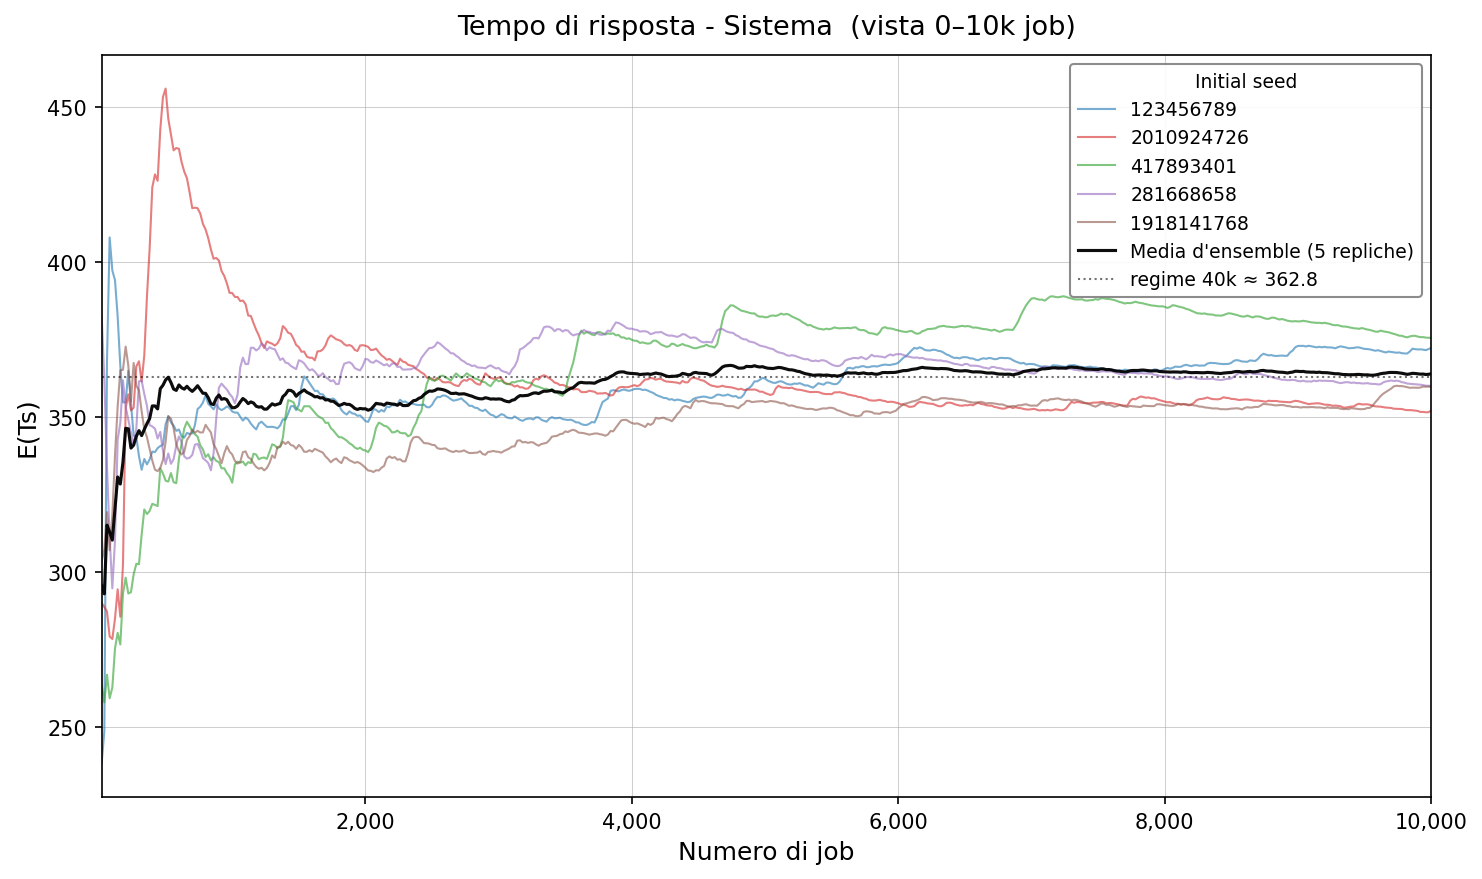
\includegraphics[width=0.85\linewidth]{images/transient_responseTime_10k.png}
    \caption{Transitorio del tempo di risposta di sistema, si mostrano i primi 10.000 job per rendere piu visibile il warm-up}
\end{figure}
\subsubsection*{Risultati}
Le curve si appiattiscono rapidamente e \emph{non divergono}: il sistema è stabile, in accordo con
la previsione operazionale. La statistica più lenta a convergere è la popolazione di sistema
($\approx 440$ completamenti); il tempo di risposta si assesta dopo $\approx 320$ e
l'utilizzazione dopo $\approx 240$. I valori di regime,  tempo di risposta $\approx 363$ s,
utilizzazione casse $\approx 0{,}47$, $\mathbb{E}[N] \approx 7{,}4$,  sono coerenti con il
flusso forzato e con le stime di batch means della sezione di verifica ($357{,}8 \pm 6{,}2$ s).

Per le run a orizzonte infinito si adotta un \textbf{warm-up di 1\,000 job}, oltre venti volte la
stima: la scelta, deliberatamente cautelativa, costa una frazione trascurabile del tempo di
simulazione e mette la stima steady-state al riparo da ogni residuo di bias iniziale.

\subsection{Calibrazione della batch size}
\schedaattivita{2}{infinito (preparatoria)}%
{quale dimensione di batch $b$ rende i batch means (quasi) indipendenti, e quindi affidabili gli
intervalli di confidenza di tutte le run a orizzonte infinito?}%
{$b = 1024$ con $k = 64$ (test di Chatfield: $\max|r_1| = 0{,}194 < 0{,}25$, conferme
multi-seed), adottata in tutte le run a orizzonte infinito dello studio.}
\begin{multicols}{2}
La scelta di $(b,k)$ non cambia la stima puntuale ma la validità dell'intervallo di confidenza: i
batch means devono essere approssimativamente scorrelati. Fissato $k = 64$ (il valore raccomandato
dal corso, $\ge 32$), la dimensione $b$ è cercata \textbf{per raddoppio}: si parte da $b = 1024$ e
si raddoppia finché l'autocorrelazione lag-1 delle serie di batch means non scende sotto la soglia
di Chatfield $2/\sqrt{k} = 0{,}25$, con un margine prudenziale del 20\% ($|r_1| \le 0{,}20$) e
conferma su seed aggiuntivi. Il test è quello contenuto nella libreria
(\texttt{Acs}): si controlla il solo lag-1 perché, a $b$ grande, la correlazione residua tra batch
adiacenti domina quella ai lag superiori,  il lag-1 è quindi un proxy sufficiente
dell'indipendenza.
\end{multicols}
\newpage
\subsection{La baseline: la gestione attuale}
\schedaattivita{3}{finito (128 repliche)}%
{quanto costa e che qualità di servizio offre la gestione attuale, 5 casse e 2 magazzinieri per
tutta la giornata, inventario con regola prudenziale uniforme e revisione delle scorte ogni 60
minuti?}%
{riferimento del confronto: $3\,561$ \euro/giorno (di cui $1\,569$ di sole perdite d'inventario),
$P(\text{OOS}) = 11{,}1\%$ --- che \emph{viola} il vincolo del 5\% --- $\mathbb{E}[T] = 333$ s;
gestione deficitaria tanto sul costo quanto sul servizio.}
\begin{multicols}{2}
\subsubsection*{Scenario e scelta dell'orizzonte}
La baseline riproduce la gestione corrente della farmacia: \textbf{5 casse e 2 magazzinieri}
attivi dall'apertura alla chiusura, inventario governato dalla regola uniforme prudenziale
$s = \{60,55,45,45,25\}$, circa il $75$--$80\%$ della capacità $S$ per ogni classe e
\textbf{revisione delle scorte ogni 60 minuti}. È l'impostazione ``di buon senso'' tipica di una
gestione non ottimizzata: soglie uguali per tutte le classi, apparentemente alte, e un controllo
delle giacenze poco frequente affidato all'operatore.

L'orizzonte è \textbf{finito} per necessità, non per convenzione: la baseline deve essere misurata
nelle condizioni in cui il sistema vive davvero, la giornata 08:00--20:00 con il profilo NSPP,
il banco pieno all'apertura, i picchi che si formano e si riassorbono, perché è su quella
giornata che si formano i costi e si giudicano i vincoli. 128 repliche indipendenti, intervalli di
confidenza al 95\%, statistiche per finestra da 30 minuti lungo la giornata.
\end{multicols}

\begin{center}

\includegraphics[width=0.49\textwidth]{images/baseline/baseline_system_response.png}\hfill

\includegraphics[width=0.49\textwidth]{images//baseline/baseline_casse_util.png}\\[0.6em]

\includegraphics[width=0.49\textwidth]{images//baseline/baseline_bracciodue_util.png}\hfill

\includegraphics[width=0.49\textwidth]{images//baseline/baseline_carico_util.png}
\end{center}
\textit{\small Figura: Baseline tempo di risposta e utilizzazione farmacisti; utilizzazione Braccio Due e coda di carico.}

\newpage
\subsubsection*{Risultati e commento}
\begin{multicols}{2}
Sul piano \textbf{economico} il quadro è pesante: $1\,992$ \euro/giorno di personale e ben
$1\,569$ \euro/giorno di inventario, per un totale di $3\,561$ \euro/giorno. Il dato che salta
all'occhio è il costo d'inventario, quasi pari a quello del personale: non è giacenza,
che con soglie alte è modesta, ma \textbf{shortage cost}, le vendite perse per out-of-stock.
La gestione baseline, cioè, brucia in perdite di servizio quasi quanto spende in stipendi.

Sul piano del \textbf{servizio} il vincolo non è rispettato: $P(\text{OOS}) = 11{,}1\%$, oltre il
doppio della soglia del 5\%, con $258$ articoli persi su $2\,324$ domandati. La causa è strutturale
e vale la pena isolarla, perché è il filo che guida tutta l'ottimizzazione. \textbf{Le cinque casse
sempre attive lavorano a utilizzazione bassa ($0{,}3$--$0{,}6$)}: lontane dalla saturazione, non
trattengono il flusso e riversano sui Bracci l'intera domanda, picchi compresi. Lo si legge negli
interarrivi: nelle fasce di punta un ordine raggiunge il \textbf{Braccio Due} in media ogni
$\approx 50$ s, contro i $\approx 118$ s del primo mattino. Ma
i Bracci sono una \textbf{risorsa a capacità fissa}, e la catena di rifornimento non riesce a ricostituire le scorte al ritmo con cui il picco le
consuma: il banco si svuota e si generano gli out-of-stock. A questo si aggiunge, come concausa, la
\textbf{revisione delle scorte ogni 60 minuti}: il riordino scatta di rado e il delivery lag medio
di $35$ minuti ritarda ulteriormente il ripristino, così che le classi ad alta rotazione restano
scoperte proprio durante i picchi. Il tempo di risposta end-to-end è $\mathbb{E}[T] = 333$ s
($\approx 5{,}5$ minuti dall'ingresso in coda alla cassa all'uscita dal pagamento).

Sul piano dell'\textbf{efficienza}, infine, la baseline mostra il secondo margine che la Fase II
recupera: le casse a $0{,}3$--$0{,}6$ significano che per gran parte della giornata cinque
farmacisti servono una domanda da due o tre, mentre i Bracci robotici lavorano a $0{,}7$--$0{,}8$
nei picchi. Il collo del sistema è dunque il robot (capacità fissa), non le casse (leva di costo):
ed è proprio qui che le due leve si saldano. Ridurre e turnare le casse non taglia soltanto il costo
del personale, ma \textbf{regola anche la frequenza con cui i job raggiungono i bracci},
alleggerendo i picchi sulla catena di rifornimento; e affiancare a questo una revisione delle scorte
più frequente e soglie differenziate per classe completa il recupero dell'out-of-stock.
\end{multicols}
\begin{figure}[h]
    \centering
    
\includegraphics[width=\linewidth]{images/baseline/inventory_combinato.png}
    \caption{Livello dell'inventario nell'unità di tempo, ogni colore rappresenta una classe di farmaci.}
\end{figure}

\newpage
\section{Fase II,  L'ottimizzazione}
\begin{multicols}{2}
Con la baseline come riferimento, la seconda fase agisce sulle due leve dichiarate negli
obiettivi, in un ordine preciso: \textbf{prima l'inventario}, \textbf{poi lo staffing}, quindi la
\textbf{ricomposizione} delle due scelte sulla giornata reale e il
\textbf{confronto economico finale} . Le prime due attività \emph{scelgono}, 
ciascuna sull'orizzonte adatto alla propria domanda,  le ultime tre \emph{verificano e
quantificano} sull'orizzonte finito. La verifica congiunta finale non è una formalità: il lead
time di rifornimento è endogeno e dipende anche dallo staffing , quindi la coppia inventario+staffing va sempre rivalidata insieme, ed è ciò che le
attività successive fanno.
\end{multicols}

\subsection{La politica di riordino $(s,S)$}
\schedaattivita{4}{finito (16 repliche CRN per configurazione)}%
{quali soglie di riordino $s_c$ per classe, quale periodo di revisione $R$ e quale livello
iniziale minimizzano il costo d'inventario rispettando $P(\text{OOS}) \le 5\%$ sulla giornata?}%
{$s = \{75,65,55,40,30\}$, $R = 30$ min, banco pieno all'apertura: $P(\text{OOS}) = 3{,}36\%$
(minimo osservato), $\approx 675$ \euro/giorno, Pareto-ottima; $R = 60$ min scartato (infeasible).}
\begin{multicols}{2}
La prima leva di ottimizzazione è la politica d'inventario: le soglie di riordino $s_c$ per
classe, il periodo di revisione $R$ e il livello iniziale del banco. Le capacità $S_c$ sono
\emph{fisse} (vincolo fisico del banco robotizzato).

\subsubsection*{Metodo}
Lo spazio esplorato è una griglia sulle soglie per classe, incrociata con
$R \in \{30, 60\}$ minuti e livello iniziale $f\cdot S$ con $f \in \{0{,}85,\ 1{,}0\}$: 576
configurazioni. Ogni configurazione è valutata con \textbf{16 repliche} della giornata a orizzonte
finito (profilo NSPP completo, personale pieno, common random numbers), catturando
$P(\text{OOS})$, costo d'inventario, tempo di risposta e delivery lag. Si è scelto l'orizzonte
finito perché la politica deve reggere il \emph{profilo} giornaliero,  i picchi consumano il
banco più della media,  e perché il costo d'inventario è naturalmente definito sulla giornata.
Nessuna funzione di merito aggregata: la selezione avviene sul \textbf{fronte di Pareto}
costo--$P(\text{OOS})$.

\subsubsection*{Risultati}
Il confronto tra i periodi di revisione è netto: con $R = 60$ minuti nessuna configurazione
rispetta il vincolo ($P(\text{OOS})$ minimo $\approx 11\%$) e i costi, dominati dallo shortage,
raddoppiano,  il banco, con i suoi buffer da poche decine di unità per classe, non copre
un'ora di domanda di picco. \textbf{$R = 30$ minuti} è quindi il periodo adottato, e su di esso
un ampio insieme di configurazioni soddisfa il vincolo del 5\%.

Sul fronte di Pareto la configurazione scelta è
\[
s = \{75,\ 65,\ 55,\ 40,\ 30\}, \qquad R = 30 \text{ min},
\]
che realizza il \textbf{minimo $P(\text{OOS})$ osservato ($3{,}36\%$)} con costo d'inventario
$\approx 675$ \euro/giorno, ad appena $+0{,}7\%$ dal minimo di costo assoluto: nessuna
configurazione è contemporaneamente più economica e con meno perdite (Pareto-ottima). Rispetto
alla regola uniforme di partenza ($s \approx 75\text{--}80\%$ di $S$ per tutte le classi), la
ricerca \emph{differenzia per classe}: porta la copertura delle classi 1--3 e 5 vicino alla
capacità ($s/S \approx 0{,}86\text{--}0{,}94$) e trattiene la classe 4 ($s_4/S_4 \approx 0{,}73$)
,  coerentemente con la lettura ``a guardrail'' del modello di costo: si compra copertura dove il
rischio di stockout durante il lead time la richiede, non ovunque. Il tempo di risposta di sistema
è risultato, come atteso, insensibile alla politica d'inventario (la variabile agisce sulle
perdite, non sulle code dei clienti).

Sul \emph{delivery lag} va registrato un aspetto strutturale: il lag medio ($\approx 23$ minuti) è
inferiore a $R$, ma nei burst di riordino,  quando più classi scattano alla stessa revisione, 
circa un quarto degli ordini completa il carico oltre la revisione successiva (massimo osservato
$\approx 59$ minuti). La regola del singolo ordine pendente per classe impedisce l'accumulo (il
riordino successivo della classe attende il completamento del precedente) e il $P(\text{OOS})$
resta entro il vincolo: si è quindi assunto come criterio operativo il livello di servizio,  Imporre ``lag mai oltre $R$'' sarebbe stato un vincolo più severo del
necessario.
\end{multicols}

\begin{figure}[h]
    \centering
    
\includegraphics[width=\linewidth]{images/inventory/inventory_search_selection.png}
    \caption{Ricerca della politica $(s,S)$: costo d'inventario contro $P(\text{OOS})$ per le
    configurazioni esplorate a $R=30$ min; la configurazione scelta (evidenziata) è
    Pareto-ottima e rispetta il vincolo del 5\% con il margine più ampio.}
\end{figure}
\FloatBarrier

\subsection{Lo staffing per fascia oraria}
\schedaattivita{5}{infinito (96 run $64 \times 1024$, una per fascia $\times$ configurazione)}%
{quante casse e quanti magazzinieri servono in ciascuna delle 12 fasce orarie, a parità
d'inventario ?}%
{profilo per fascia: 2--4 casse e 1--2 magazzinieri (mai i 5+2 attuali), personale
$1\,364$ \euro/giorno ($-31{,}5\%$); nelle 5 fasce di punta scelta best-effort .}
\begin{multicols}{2}
La seconda leva,  quella economicamente dominante,  è il numero di farmacisti  e di
magazzinieri attivi in ciascuna delle 12 fasce orarie.

\subsubsection*{Metodo}
Per ogni fascia (con $\lambda$ pari alla media dei suoi due slot da 30 minuti) e per ogni
combinazione di staffing,  casse $\in \{2,3,4,5\}$, magazzinieri $\in \{1,2\}$, 96 run in totale
,  si esegue una simulazione a \textbf{orizzonte infinito} ($64 \times 1024$ batch, warm-up
1\,000 job, inventario fisso alla configurazione scelta nella sezione precedente). Mantenere il $\lambda$ di una fascia costante per un tempo infinito
equivale a uno \textbf{stress test},  decine di giornate consecutive tutte intense come quella
fascia,  e serve a determinare, a parità di domanda, \textbf{la configurazione di costo minimo
che non diverge}.

La metrica di scelta è il \textbf{costo totale monetizzato} della fascia:
\[
C_{tot} = C_{\text{lavoro}} + C_{\text{inventario}} + C_{\text{attesa}},
\]
dove $C_{\text{lavoro}}$ usa le tariffe del modello di costo (26/18 \euro/h),
$C_{\text{inventario}}$ include holding, shortage e ordini, mentre $C_{\text{attesa}}$:
\[C_{\text{attesa}}= c_w \cdot
N_{\text{clienti}} \cdot \mathbb{E}[T_r]\] monetizza il tempo dei clienti con un \emph{valore del
tempo} $c_w = 10$ \euro/h , ordine di grandezza del 30--50\% del salario orario. Questa costruzione evita lo score a pesi arbitrari: ogni termine è in
\euro/giorno, e una configurazione che facesse esplodere le attese non può vincere
perché $C_{\text{attesa}}$ cresce linearmente in $\mathbb{E}[T_r]$.

Una configurazione è \textbf{ammissibile} se $P(\text{OOS}) \le 5\%$ \emph{e} se è
\textbf{stabile}, ovvero se il throughput misurato regge la domanda offerta ($X \ge 0{,}9\,
\lambda$). Il filtro di stabilità è essenziale e non ovvio: nelle fasce calde le configurazioni
sotto-dimensionate mostrano $P(\text{OOS})$ \emph{artificialmente basso},  con le casse sature
la domanda resta bloccata in coda e non raggiunge mai il banco. Nella fascia 18--19, ad esempio, il $P(\text{OOS})$ minimo assoluto
($0{,}11\%$) appartiene a una configurazione instabile, mentre la migliore configurazione
\emph{stabile} è al $12{,}5\%$. Tra le ammissibili si sceglie il minimo $C_{tot}$; dove nessuna
configurazione è ammissibile si adotta la migliore per costo tra quelle stabili
(\emph{best-effort}).
\end{multicols}

\begin{table}[ht]
\centering
\renewcommand{\arraystretch}{1.2}
\begin{tabular}{|c|c|r|r|r|c|c|c|}
\hline
\textbf{Fascia} & \textbf{(casse, mag)} & $\mathbb{E}[T_r]$ (s) & $P(\text{OOS})$ &
$C_{tot}$ (\euro) & $\rho_{\text{casse}}$ & $\rho_{B1}$ & \textbf{Stato} \\
\hline
08--09 & (2,1) & 296 & 0{,}00\%  & 1341 & 0{,}52 & 0{,}34 & ammissibile \\
09--10 & (3,1) & 397 & 1{,}16\%  & 2304 & 0{,}74 & 0{,}73 & ammissibile \\
10--11 & (3,1) & 439 & 2{,}25\%  & 2561 & 0{,}79 & 0{,}77 & ammissibile \\
11--12 & (4,2) & 636 & 8{,}98\%  & 5080 & 0{,}85 & 0{,}95 & best-effort \\
12--13 & (4,2) & 542 & 6{,}35\%  & 4277 & 0{,}82 & 0{,}93 & best-effort \\
13--14 & (3,1) & 334 & 0{,}14\%  & 1976 & 0{,}65 & 0{,}62 & ammissibile \\
14--15 & (3,1) & 340 & 0{,}16\%  & 2000 & 0{,}66 & 0{,}64 & ammissibile \\
15--16 & (3,1) & 317 & 0{,}03\%  & 1905 & 0{,}61 & 0{,}58 & ammissibile \\
16--17 & (3,2) & 534 & 1{,}76\%  & 3076 & 0{,}85 & 0{,}84 & ammissibile \\
17--18 & (4,2) & 781 & 10{,}92\% & 6009 & 0{,}87 & 0{,}97 & best-effort \\
18--19 & (4,2) & 866 & 12{,}54\% & 6577 & 0{,}88 & 0{,}97 & best-effort \\
19--20 & (4,2) & 543 & 6{,}59\%  & 4322 & 0{,}82 & 0{,}93 & best-effort \\
\hline
\end{tabular}
\caption{Configurazione di staffing selezionata per fascia. Le
cinque fasce di punta sono \emph{best-effort}: nessuno staffing stabile rispetta il 5\% di
out-of-stock sotto stress prolungato.}
\end{table}

\begin{multicols}{2}
\subsubsection*{Lettura dei risultati}
Nelle fasce ordinarie bastano \textbf{2--3 casse e 1 magazziniere}, con casse a utilizzazione sana ($0{,}5$--$0{,}8$) e vincolo di servizio rispettato con
margine. Nelle \textbf{cinque fasce di punta} (11--13 e 17--20) nessuna configurazione stabile
scende sotto il 5\% di out-of-stock: aggiungere casse non aiuta,  anzi, immette domanda più in
fretta verso un banco che non riesce a ricaricarsi,  perché sotto stress prolungato satura la
\textbf{catena di rifornimento} ($\rho_{B1} \approx 0{,}93$--$0{,}97$ nella tabella), esattamente
come previsto dall'analisi del flusso forzato ($X_{\max}^{\text{carico}} \approx 0{,}023 <
\lambda_{\text{picco}}$). In quelle fasce la scelta cade sul minimo costo tra le configurazioni
stabili, (4,2), e la verifica del vincolo è rimandata,  correttamente,  alla giornata intera:
nell'orizzonte finito i picchi sono transitori di 30--60 minuti, il banco pieno li assorbe, e il
$P(\text{OOS})$ complessivo resterà sotto il 5\% .

Il profilo risultante,
\[
\text{casse} = [2,3,3,4,4,3,3,3,3,4,4,4],
\]
\[
\text{mag} = [1,1,1,2,2,1,1,1,2,2,2,2],
\]
vale $40$ ore-cassa e $18$ ore-magazziniere al giorno, cioè un costo del personale di
\[
40 \cdot 26 + 18 \cdot 18 = \textbf{1\,364 \euro/giorno}
\]
contro i $1\,992$ della gestione baseline ($-31{,}5\%$ sul personale).
\end{multicols}
\begin{figure}[htbp]
\centering

\includegraphics[width=\textwidth]{images/configsearch/configsearch_g1.png}\\[0.5em]

\includegraphics[width=\textwidth]{images/configsearch/configsearch_g2.png}\\[0.5em]

\includegraphics[width=\textwidth]{images/configsearch/configsearch_g3.png}\\[0.5em]

\includegraphics[width=\textwidth]{images/configsearch/configsearch_g4.png}
\caption{Scomposizione del costo totale $C_{tot}$ per configurazione di staffing, tutte le 12 fasce}
\label{fig:configsearch-breakdown}
\end{figure}


\subsubsection*{Dal profilo ottimo ai turni realistici}
\begin{multicols}{2}
Il profilo di staffing per fascia non è direttamente attuabile: preso alla lettera implicherebbe
contratti da una o due ore. In coda all'attività 5 il profilo viene quindi tradotto in
\textbf{turni contigui realistici} con tre regole: decomposizione del profilo in turni (chi apre
per il picco chiude a fine picco), durata minima di 3 ore,  i turni-spike sono estesi verso le
ore adiacenti a domanda più alta, producendo solo sovra-copertura,  e durata massima di 8 ore,
oltre la quale il turno è spezzato su due persone. Per costruzione la copertura oraria risultante
è \emph{sempre maggiore o uguale} allo staffing ottimo.

\end{multicols}

\newpage
\subsection{Scenario ottimizzato sulla giornata reale}
\schedaattivita{6}{finito (128 repliche)}%
{le due scelte della fase,  inventario (attività 4, deciso sul finito) e staffing (attività 5,
deciso sull'infinito),  reggono \emph{insieme} la giornata operativa completa, vincoli
compresi?}%
{sì: $2\,104$ \euro/giorno ($-22{,}8\%$ sulla baseline), $P(\text{OOS}) = 3{,}94\% \le 5\%$
sull'intera giornata, $\mathbb{E}[T] = 393$ s ($+56$ s).}
\begin{multicols}{2}
Lo scenario \textbf{Ottimizzato} ricompone le decisioni della fase: staffing a profilo
$[2,3,3,4,4,3,3,3,3,4,4,4]$ casse e $[1,1,1,2,2,1,1,1,2,2,2,2]$ magazzinieri, inventario
$s = \{75,65,55,40,30\}$ con $R = 30$ minuti. La valutazione usa la stessa identica metodologia
della baseline (128 repliche, profilo NSPP, banco pieno, stessi stream): questo passaggio
\emph{chiude il cerchio} tra i due orizzonti,  le decisioni prese a $\lambda$ costante devono
dimostrarsi valide nella giornata non stazionaria, l'unico contesto in cui i vincoli hanno
significato operativo.

I risultati confermano le scelte. Il costo scende a \textbf{$2\,104$ \euro/giorno}
($1\,364$ di personale $+ 740$ d'inventario, $-22{,}8\%$ sul totale baseline). Il punto
metodologicamente notevole è il vincolo di servizio: \textbf{$P(\text{OOS}) = 3{,}94\%$,
rispettato sull'intera giornata},  nonostante nelle cinque fasce di punta l'attività 5 non
avesse trovato alcuna configurazione ammissibile sotto stress perpetuo. È la conferma quantitativa
della divisione dei compiti tra orizzonti dichiarata nel piano: lo stress test a $\lambda$
costante serviva a \emph{scegliere} la configurazione stabile di costo minimo, non a prevedere il
servizio di giornata; nella giornata reale i picchi durano 30--60 minuti, il banco pieno li
attraversa, e le perdite restano entro il vincolo (figura). Il tempo di risposta sale a
$\mathbb{E}[T] = 392{,}5$ s ($+56$ s sulla baseline): è il prezzo, atteso, del passaggio delle
casse da sovradimensionate a dimensionate. Tutta la domanda resta servita ($810$ clienti/giorno)
e il delivery lag medio ($23$ minuti) resta entro il periodo di revisione.
\end{multicols}

\begin{center}

\includegraphics[width=0.49\textwidth]{images/ottimo/ott_system_response.png}\hfill

\includegraphics[width=0.49\textwidth]{images/ottimo/ott_casse_util.png}\\[0.6em]

\includegraphics[width=0.49\textwidth]{images/ottimo/ott_bracciodue_util.png}\hfill

\includegraphics[width=0.49\textwidth]{images/ottimo/ott_carico_util.png}
\end{center}


\begin{figure}[H]
    \centering
    
\includegraphics[width=0.9\linewidth]{images/ottimo/inventory_combinato.png}
    \label{fig:placeholder}
\end{figure}
\begin{figure}[H]
    \centering
    
\includegraphics[width=0.9\linewidth]{images/ottimo/confronto_inventario_classe2.png}
    \label{fig:placeholder}
\end{figure}


\newpage

\subsection{Scenario con turnazione realistica}
\schedaattivita{7}{finito (128 repliche)}%
{lo staffing ottimo dell'attività 6 è un profilo per fascia, non un organico:
preso alla lettera implicherebbe contratti da una o due ore. Si può tradurre in una
\emph{turnazione realmente attuabile} senza perdere il beneficio dell'ottimizzazione né
violare i vincoli?}%
{sì: $2\,131$ \euro/giorno ($-40{,}2\%$ sulla baseline), $P(\text{OOS}) = 3{,}70\%
\le 5\%$; il costo del personale sale di poco --- il prezzo del realismo --- a fronte di un
servizio che resta pieno e anzi leggermente migliore.}
\begin{multicols}{2}
L'attività 6 fornisce lo staffing \emph{ottimo per fascia oraria}, ma un
profilo di occupazione non è ancora una turnazione: applicato alla lettera richiederebbe
personale assunto per una o due ore isolate, impossibile da mettere a contratto. L'obiettivo di
questa attività è \textbf{trasformare quel profilo in una turnazione realistica e attuabile}, senza
turni-spezzone di poche ore, e rivalutarla per intero sulla giornata operativa.

È il passo che rende l'ottimizzazione
\emph{operativamente credibile}: risponde alla domanda ``la farmacia può davvero organizzare
questi turni?'' e verifica che il risparmio e i vincoli di servizio sopravvivano una volta imposti
i vincoli reali del personale (durata e continuità dei turni). È, di fatto, l'unico dei tre
scenari direttamente implementabile, e quindi quello che la trattazione può \textbf{raccomandare}
come configurazione concreta, non come risultato astratto di un'ottimizzazione.

Rendere lo staffing attuabile ha un prezzo:
coprire la domanda con turni contigui e sensati richiede qualche ora-uomo in più del minimo
teorico e il
\textbf{costo del personale cresce} (da $1\,364$ a $1\,426$ \euro/giorno). In cambio, quelle ore aggiuntive
cadono a ridosso dei picchi, e il \textbf{servizio migliora}: il costo d'inventario scende a
$705$ \euro, l'out-of-stock è il più basso dei tre scenari ($3{,}70\%$) e il tempo di risposta
scende a $\mathbb{E}[T] = 377$ s. Alcuni indicatori peggiorano (il costo), altri migliorano (il
servizio): il modesto aumento di spesa è esattamente \textbf{il prezzo da pagare per una
configurazione realistica}.
\end{multicols}

\begin{figure}[h]
    \centering
    
\includegraphics[width=\linewidth]{images/turni_realistici_8h.png}
    \caption{Turnazione realistica derivata dallo staffing ottimo}
\end{figure}
\FloatBarrier

\newpage
\subsection{Confronto finale dei tre scenari}
\schedaattivita{8}{analisi comparativa delle attività}%
{quanto si risparmia rispetto alla gestione baseline, e a quale prezzo sulle prestazioni percepite
dal cliente?}%
{la gestione baseline è deficitaria su due fronti: costa troppo \emph{e} viola il vincolo di
servizio ($P(\text{OOS}) = 11{,}12\%$). L'ottimizzazione li risolve insieme: $-40{,}2\%$ di costo
($\approx 436\,000$ \euro/anno) nello scenario raccomandato con turni realistici, out-of-stock
riportato a $3{,}70\% \le 5\%$, al prezzo di $+44$ s di tempo di risposta.}

Il confronto finale affianca i tre scenari valutati nelle attività 3, 6 e 7  tutti sulla stessa
giornata a orizzonte finito, con le stesse 128 repliche e gli stessi stream , quindi confrontabili riga per riga. La tabella riassume i numeri già discussi nelle
rispettive attività; qui se ne dà la lettura economica e di servizio complessiva, insieme al
confronto lungo la giornata.


\begin{table}[ht]
\centering
\renewcommand{\arraystretch}{1.3}
\begin{tabular}{|l|r|r|r|r|r|r|}
\hline
\textbf{Scenario} & \textbf{Personale} & \textbf{Inventario} & \textbf{Totale}
& $\Delta$ \textbf{costo} & $P(\text{OOS})$ & $\mathbb{E}[T]$ \\
 & (\euro/gg) & (\euro/gg) & (\euro/gg) & & & (s) \\
\hline
Baseline            & 1\,992 & 1\,569 & \textbf{3\,561} & ---        & 11{,}12\% & 333 \\
Ottimizzato         & 1\,364 & 740    & \textbf{2\,104} & $\mathbf{-40{,}9\%}$ & 3{,}94\% & 393 \\
Ottimizzato + turni & 1\,426 & 705    & \textbf{2\,131} & $\mathbf{-40{,}2\%}$ & 3{,}70\% & 377 \\
\hline
\end{tabular}
\caption{Confronto economico e di servizio dei tre scenari sulla giornata operativa}
\end{table}

\begin{multicols}{2}
\subsubsection*{Lettura economica}
Il costo giornaliero scende da $3\,561$ \euro{} della gestione baseline a $2\,131$ \euro{} dello
scenario con turni realistici: $\mathbf{-40{,}2\%}$, circa $-1\,430$ \euro/giorno, che su circa
305 giorni operativi valgono \textbf{$\approx 436\,000$ \euro/anno}. Il risparmio non viene solo
dal personale ($-566$ \euro/giorno per il dimensionamento delle casse): una quota persino maggiore
($-864$ \euro/giorno) viene dal \textbf{costo d'inventario}, perché nella baseline quella voce è
dominata dallo \emph{shortage}. Non è l'inventario
usato come leva di risparmio: è la baseline che, con revisione
lenta ($R = 60$ min) e soglie basse, paga uno shortage evitabile che la politica ottimizzata
($R = 30$, soglie più alte) azzera. Fra i due scenari \emph{già} ottimizzati, infatti, il costo
d'inventario è pressoché invariato ($705$--$740$ \euro), a conferma del suo ruolo di guardrail una
volta dentro la regione ammissibile.\\La versione con \textbf{turni realistici} costa $27$ \euro/giorno più dell'ottimo puro
($+1{,}3\%$): la sovra-copertura richiesta da turni contrattualmente sensati non erode il
risparmio, e le ore aggiuntive a ridosso dei picchi le fanno anzi ottenere il $P(\text{OOS})$
migliore dei tre scenari ($3{,}70\%$). È lo scenario raccomandato: l'unico direttamente attuabile,
a costo praticamente uguale all'ottimo teorico.

\subsubsection*{Lettura del servizio}
Il dato più netto è che la \textbf{gestione baseline viola il vincolo di servizio}:
$P(\text{OOS}) = 11{,}12\%$, oltre il doppio della soglia del $5\%$. La causa non sono le casse ma
la politica d'inventario, con revisione ogni $60$ minuti la scorta si esaurisce tra due
revisioni nelle fasce di domanda alta. Entrambi gli scenari ottimizzati \textbf{ristabiliscono il
vincolo} ($3{,}94\%$ e $3{,}70\%$) grazie alla revisione a $30$ minuti e alle soglie più alte sulle
classi critiche: l'ottimizzazione, quindi, non si limita a tagliare i costi, \textbf{ripara anche
il servizio}.

Il prezzo è sul \textbf{tempo di risposta}: da $333$ a $377$ secondi end-to-end nello scenario
raccomandato ($+44$ s, $+13\%$; $+60$ s per l'ottimo puro), cioè da $5{,}5$ a $6{,}3$ minuti
sull'intero percorso cassa--robot--pagamento. L'aumento è l'effetto atteso del passaggio delle
casse da sovradimensionate ($\rho \approx 0{,}3$--$0{,}6$) a dimensionate
($\rho \approx 0{,}6$--$0{,}9$), è distribuito lungo la giornata senza esplosioni nelle fasce di
punta (figura), e i turni realistici, con la copertura extra a ridosso delle ore critiche, lo
contengono meglio dell'ottimo puro ($377$ contro $393$ s). Un minuto in più di permanenza a fronte
di due quinti di costo in meno e di un servizio riportato entro QoS è il termine di scambio che
lo studio quantifica e consegna alla decisione del gestore.
\end{multicols}
\subsubsection*{Cosa non cambia}
\begin{multicols}{2}
Le utilizzazioni dei bracci robotici e del percorso di rifornimento sono sostanzialmente invariate
tra gli scenari: lo staffing non tocca il robot (capacità fissa) e il throughput è conservato ---
tutta la domanda è servita in ogni scenario ($810$ clienti/giorno, abbandoni disattivati). Questo
conferma che l'ottimizzazione ha agito solo sulle leve dichiarate (turni e politica d'inventario),
senza effetti collaterali nascosti sul cuore automatizzato del sistema.
\end{multicols}

\begin{center}

\includegraphics[width=0.8\textwidth]{images/confronto/system_Response.png}\\[0.6em]

\includegraphics[width=0.8\textwidth]{images/confronto/Casse Farmacia_Utilization.png}\\[0.6em]

\includegraphics[width=0.8\textwidth]{images/confronto/Braccio Uno Carico_Utilization.png }\\[0.6em]  

\includegraphics[width=0.8\textwidth]{images/confronto/Braccio Due_Utilization.png}
\end{center}
\newpage
\section{Conclusioni}
\begin{multicols}{2}
Lo studio ha modellato una farmacia con dispensazione robotizzata Gollmann come rete di code con
inventario integrato, l'ha verificata e validata, e ne ha ottimizzato la gestione operativa a
parità di architettura. L'obiettivo dichiarato,  ridurre i costi di esercizio senza degradare il
servizio,  è raggiunto con un margine più ampio del previsto, perché l'analisi ha rivelato che la
gestione baseline non solo costa troppo ma \textbf{viola essa stessa il vincolo di servizio}
($P(\text{OOS}) = 11{,}12\%$, oltre il doppio della soglia del $5\%$, per effetto della revisione
lenta a $R = 60$ min). Lo scenario raccomandato con turni realistici risolve entrambi i problemi
insieme: \textbf{$-40{,}2\%$ di costo giornaliero} ($\approx 436\,000$ \euro/anno), out-of-stock
riportato entro l'SLA ($3{,}70\% \le 5\%$) e un aumento contenuto del tempo di risposta
($+44$ s, $+13\%$, circa tre quarti di minuto sul percorso end-to-end). L'ottimizzazione, quindi,
non taglia i costi a spese del servizio: li taglia \emph{riparando} anche il servizio, perché il
passaggio a $R = 30$ min con soglie più alte sulle classi critiche è a sua volta una delle leve
individuate dallo studio.

Il percorso metodologico ha seguito l'ordine prescritto: modello concettuale e delle specifiche,
analisi operazionale del flusso forzato, verifica (bilanci esatti, leggi di Little, accordo con
$M/M/1$, $M/M/2$ e Pollaczek--Khinchine entro gli intervalli di confidenza, test degenerato
dell'inventario con match esatto sul riferimento del corso), validazione (plausibilità, check di
flusso, sensitività alle assunzioni distributive), quindi il \textbf{piano sperimentale in otto
attività su due fasi},  prima il sistema attuale (transitorio, calibrazione dei batch,
baseline), poi l'ottimizzazione (inventario, staffing, scenari ottimizzati, confronto),  con
l'orizzonte di simulazione dichiarato e motivato attività per attività: \textbf{finito} (128
repliche della giornata NSPP) per baseline, ricerca d'inventario e scenari; \textbf{infinito}
(batch means $64 \times 1024$, Chatfield superato con $b = 1024$, warm-up $1\,000$ job) per la
stima del warm-up, la calibrazione e il ranking dello staffing a parità di domanda.

Alcune \textbf{scelte di simulazione} si sono rivelate strutturanti e meritano di essere
richiamate con il loro esito. ``Un ordine = un job'' ha eliminato il fork--join e reso veritiere le
utilizzazioni; il routing probabilistico fisso con finestra protetta ha reso la rete analizzabile
per centro (le quote effettive $0{,}133/0{,}867$ sono confermate dalle utilizzazioni misurate);
la priorità ai prelievi sul Braccio Uno ha allineato i tempi dei clienti sui due bracci; la
politica lost-sales ha ancorato la metrica di servizio al comportamento reale del cliente di
farmacia; la disattivazione degli abbandoni ha isolato il sottosistema d'inventario dandogli una
domanda ben definita; il cap dei picchi a $0{,}0255$ req/s ha mantenuto il collo di bottiglia dei
clienti (Braccio Due) entro $\rho = 0{,}95$.

Il risultato concettualmente più interessante riguarda il \textbf{ruolo dell'inventario}:
l'asimmetria dei costi ($\approx 500\times$ tra shortage e giacenza) lo rende un guardrail, non
una leva di risparmio, e l'analisi del flusso forzato mostra che sotto domanda di picco sostenuta
il primo limite del sistema è la \textbf{catena di rifornimento} ($X_{\max} \approx 0{,}023$
req/s), non le casse: nessuno staffing può comprare livelli di servizio che il carico del robot
non riesce a sostenere. Nella giornata reale i picchi sono transitori e il banco li assorbe, 
ma è questo vincolo, non il costo del personale, a porre il pavimento sotto il quale lo staffing
non può scendere.

\subsubsection*{Limiti e sviluppi futuri}
Tre estensioni naturali restano fuori dallo scope. (i) \emph{De-burst delle revisioni}: scaglionare
le revisioni delle cinque classi con offset temporali romperebbe i burst di riordino che oggi
producono le code al carico e i lag oltre $R$, accorciando il lead time nei picchi a throughput
invariato. (ii) \emph{Disciplina del carico stato-dipendente}: servire i carichi in ordine di
urgenza di scorta (prima la classe più vicina allo stockout) anziché FIFO ridurrebbe gli
out-of-stock ``di tempismo'' a costo zero, essendo il lavoro totale conservato; da valutare per
confronto simulativo a parità di stream. (iii) \emph{Riattivazione degli abbandoni}: reintrodurre
il reneging permetterebbe di studiare l'interazione tra pazienza dei clienti e staffing ridotto,
completando il quadro del trade-off servizio--costo. Sul piano strumentale, la misura del delivery
lag andrebbe raffinata da per-ordine a per-confezione, coerente con il carico incrementale.
\end{multicols}
\newpage
\begin{thebibliography}{9}

\bibitem{leemis}
L.~M. Leemis, S.~K. Park, \textit{Discrete-Event Simulation: A First Course}, Pearson Prentice
Hall, 2006.

\bibitem{parkmiller}
S.~K. Park, K.~W. Miller, \textit{``Random Number Generators: Good Ones Are Hard to Find''},
Communications of the ACM, vol.~31, no.~10, pp.~1192--1201, 1988.

\bibitem{little}
J.~D.~C. Little, \textit{``A Proof for the Queuing Formula: $L = \lambda W$''}, Operations
Research, vol.~9, no.~3, pp.~383--387, 1961.

\bibitem{kingman}
J.~F.~C. Kingman, \textit{``The Single Server Queue in Heavy Traffic''}, Mathematical Proceedings
of the Cambridge Philosophical Society, vol.~57, no.~4, pp.~902--904, 1961.

\bibitem{chatfield}
C.~Chatfield, \textit{The Analysis of Time Series: An Introduction}, 6th ed., Chapman \&
Hall/CRC, 2003.

\bibitem{harchol}
M.~Harchol-Balter, \textit{Performance Modeling and Design of Computer Systems: Queueing Theory in
Action}, Cambridge University Press, 2013.

\bibitem{kurkowski}
S.~Kurkowski, T.~Camp, M.~Colagrosso, \textit{``MANET Simulation Studies: The Incredibles''}, ACM
SIGMOBILE Mobile Computing and Communications Review, vol.~9, no.~4, pp.~50--61, 2005.

\bibitem{denitto}
V.~de Nitto Personè, \textit{Dispense del corso di Performance Modeling of Computer Systems and
Networks}, Università degli Studi di Roma Tor Vergata, a.a. 2025/2026.

\end{thebibliography}

\end{adjustwidth}
\end{document}
